\chapter{Tools}

This chapter provides a overview of the various tools that are
provided as part of the Ames Stereo Pipeline, and a summary of their
command line options.

\section{stereo}
\label{stereo}

The \texttt{stereo} program is the primary tool of the Ames Stereo
Pipeline. It takes a stereo pair of images that overlap and creates an
output point cloud image that can be processed into a visualizable mesh
or a DEM using \texttt{point2mesh} (section \ref{point2mesh}) and
\texttt{point2dem} (section \ref{point2dem}), respectively.

\medskip

Usage:
\begin{verbatim}
  ISIS 3> stereo [options] <images> [<cameras>] output_file_prefix
\end{verbatim}

Example (for ISIS):
\begin{verbatim}
  stereo file1.cub file2.cub results/run
\end{verbatim}
For ISIS, a .cub file has both image and camera information, as such
no separate camera files are specified.

Example (for Digital Globe Earth images):
\begin{verbatim}
  stereo file1.tif file2.tif file1.xml file2.xml results/run
\end{verbatim}

Multiple input images are also supported (section \ref{multiview}).

This tool is is primarily designed to process USGS ISIS \texttt{.cub}
files and Digital Globe data. However, Stereo Pipeline
does have the capability to process other types of stereo image pairs
(e.g., image files with a CAHVOR camera model from the NASA MER
rovers). If you would like to experiment with these features, please
contact us for more information.

The \texttt{\textit{output\_file\_prefix}} is prepended to all
output data files.  For example, setting \texttt{\textit{output\_file\_prefix}}
to `\texttt{out}' will yield files with names like \texttt{out-L.tif}
and \texttt{out-PC.tif}.  To keep the Stereo Pipeline results organized
in sub-directories, we recommend using an output prefix like
`\texttt{results-10-12-09/out}' for \texttt{\textit{output\_file\_prefix}}.  The
\texttt{stereo} program will create a directory called
\texttt{results-10-12-09/} and place files named \texttt{out-L.tif},
\texttt{out-PC.tif}, etc. in that directory.

\begin{longtable}{|l|p{7.5cm}|}
\caption{Command-line options for stereo}
\label{tbl:stereo}
\endfirsthead
\endhead
\endfoot
\endlastfoot
\hline
Option & Description \\ \hline \hline
\texttt{-\/-help|-h} & Display the help message\\ \hline
\texttt{-\/-session-type|-t \textit{string} } & Select the stereo session type to use for processing. Usually the program can select this automatically by the file extension. Options: pinhole isis dg rpc spot5 aster pinholemappinhole isismapisis dgmaprpc rpcmaprpc astermaprpc. \\ \hline
\texttt{-\/-stereo-file|-s \textit{filename(=./stereo.default)}} & Define the stereo.default file to use.\\ \hline
\texttt{-\/-entry-point|-e integer(=0 to 4)} & Stereo Pipeline entry
point (start at this stage). \\ \hline
\texttt{-\/-stop-point|-e integer(=1 to 5)} & Stereo Pipeline stop point (stop at the stage {\it right before} this value). \\ \hline
\texttt{-\/-corr-seed-mode integer(=0 to 3)} & Correlation seed strategy (section \ref{corr_section}). \\ \hline
\texttt{-\/-threads \textit{integer(=0)}} & Set the number of threads to use. 0 means use as many threads as there are cores.\\ \hline
\texttt{-\/-no-bigtiff} & Tell GDAL to not create bigtiffs.\\ \hline
\texttt{-\/-tif-compress None|LZW|Deflate|Packbits} & TIFF compression method.\\ \hline
\end{longtable}

More information about additional options that can be passed to \texttt{stereo}
via the command line or via the \texttt{stereo.default} configuration file can be
found in Appendix \ref{ch:stereodefault} on page
\pageref{ch:stereodefault}.  \texttt{stereo} creates a set
of intermediate files, they are described in Appendix
\ref{chapter:outputfiles} on page \pageref{chapter:outputfiles}.

\subsection{Entry Points}
\label{entrypoints}

The \texttt{stereo -e \textit{number}} option can be used to restart
a {\tt stereo} job partway through the stereo correlation process.
Restarting can be useful when debugging while iterating on {\tt
stereo.default} settings.

Stage 0 (Preprocessing) normalizes the two images and aligns them
by locating interest points and matching them in both images. The
program is designed to reject outlying interest points.  This stage
writes out the pre-aligned images and the image masks.

Stage 1 (Disparity Map Initialization) performs pyramid correlation and builds a rough disparity map that is used to seed the sub-pixel refinement phase.

Stage 2 (Sub-pixel Refinement) performs sub-pixel correlation that
refines the disparity map.

Stage 3 (Outlier Rejection and Hole Filling) performs filtering of the
disparity map and (optionally) fills in holes using an inpainting
algorithm.  This phase also creates a ``good pixel'' map.

Stage 4 (Triangulation) generates a 3D point cloud from the disparity
map.

\subsection{Decomposition of Stereo}
\label{stereo_dec}

The \texttt{stereo}
executable is a python script that makes calls to separate
C++ executables for each entry point.

Stage 0 (Preprocessing) calls \texttt{stereo\_pprc}. Multi-threaded.

Stage 1 (Disparity Map Initialization) calls
\texttt{stereo\_corr}. Multi-threaded.

Stage 2 (Sub-pixel Refinement) class \texttt{stereo\_rfne}. Multi-threaded.

Stage 3 (Outlier Rejection and Hole Filling) calls
\texttt{stereo\_fltr}. Multi-threaded.

Stage 4 (Triangulation) calls \texttt{stereo\_tri}. Multi-threaded,
except for ISIS input data.

All of the sub-programs have the same interface as
\texttt{stereo}. Users processing a large number of stereo pairs on a
cluster may find it advantageous to call these executables in their own
manner. An example would be to run stages 0-3 in order for each stereo
pair. Then run several sessions of \texttt{stereo\_tri} since it is
single-threaded for ISIS.

It is important to note that each of the C++ stereo executables invoked
by \texttt{stereo} have their own command-line options. Those options
can be passed to \texttt{stereo} which will in turn pass them to the
appropriate executable. By invoking each executable with no options, it
will display the list of options it accepts.

As explained in more detail
in section \ref{perform-stereo}, each such option has the same syntax as
used in \texttt{stereo.default}, while being prepended by a double hyphen
(\texttt{-\/-}).  A command line option takes precedence over the same
option specified in \texttt{stereo.default}. Chapter \ref{ch:stereodefault}
documents all options for the individual sub-programs.

Note that the stereo tools operate only on single channel (grayscale) images.
If you need to run stereo on multi-channel images you must first convert them
to grayscale or extract a single channel to operate on.

\section{stereo\_gui}
\label{stereo_gui}

The \texttt{stereo\_gui} program is a GUI frontend to \texttt{stereo},
and has the same command-line options. It can display the input images
side-by-side (and in other ways, as detailed later). One can zoom in by
dragging the mouse from upper-left to lower-right, and zoom out via the
reverse motion.

By pressing the \texttt{Control} key while dragging the mouse, regions
can be selected in the input images, and then stereo can be run on these
regions from the menu via Run$\rightarrow$Stereo. The \texttt{stereo}
command that is invoked (with appropriately populated parameter values
for \texttt{-\/-left-image-crop-win} and \texttt{-\/-right-image-crop-win}
for the selected regions) will
be displayed on screen, and can be re-run on a more powerful
machine/cluster without GUI access.

Additional navigation options are using the mouse wheel or the +/- keys to
zoom, and the arrow keys to pan (one should first click to bring into
focus the desired image before using any keys).

\begin{figure}[h!]
\begin{center}
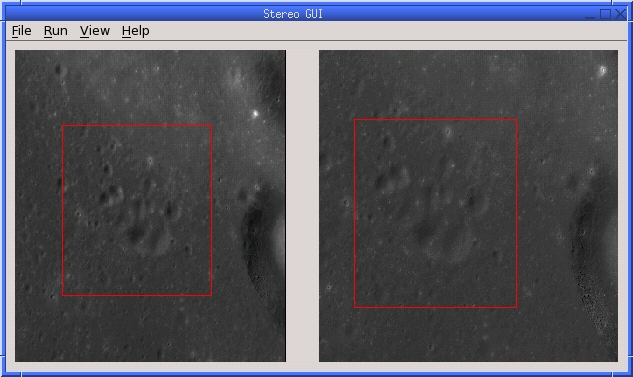
\includegraphics[width=5in]{images/stereo_gui.jpg}
\caption[asp\_gui]{An illustration of stereo\_gui. The \texttt{stereo} command
will be run on the regions selected by red rectangles.}
\label{asp_gui_fig}
\end{center}
\end{figure}

Usage:
\begin{verbatim}
  ISIS 3> stereo_gui [options] <images> [<cameras>] output_file_prefix
\end{verbatim}

\subsection{Use as an Image Viewer}

This program can be also used as a general-purpose image viewer, case in
which no stereo options or camera information is necessary.  It can
display arbitrarily large images with integer, floating-point, or RGB
pixels, including ISIS .cub files and DEMs. It handles large images by
building on disk pyramids of increasingly coarser subsampled images and
displaying the subsampled versions that are appropriate for the current
level of zoom.

The images can be shown either side-by-side, as tiles on a grid (using
\texttt{-\/-grid-cols integer}), or on top of each other (using
\texttt{-\/-single-window}), with a dialog to choose among them.  In the
last usage scenario, the option \texttt{-\/-use-georef} will overlay the
images correctly if georeference information is present.  It is possible
to switch among these modes once the GUI has been open, from the GUI
View menu.

When the images are shown side-by-side, the GUI can zoom
in all images to the same region, for easier comparison among them.

When the images are in a single window, an individual image can be turned
on or off via a checkbox. Clicking on an image's name will zoom to it
and display it on top of other images. By right-clicking the list
of images, other operations can be performed, such as deleting an image
from the view, etc. 

\texttt{stereo\_gui} can show hillshaded DEMs, either via the
\texttt{-\/-hillshade} option, or by choosing from the GUI View menu the
\texttt{Hillshaded images} option.

This program can also display the output of the ASP \texttt{colormap}
tool (section \ref{sec:colormap}).

When clicking on a pixel, the pixel indices and value will be printed on screen.
When selecting a region by pressing the \texttt{Control} key while dragging the mouse, 
its bounds will be displayed on screen. If the image is geo-referenced,
the extent of the region in projected coordinates and in the longitude-latitude domain 
will be shown as well. 

The program can also save a screenshot to disk in the BMP or XPM format. 

\subsection{Other Functionality}

\subsubsection{View/create/delete/save interest point matches}

\texttt{stereo\_gui} can be used to view interest point matches
(\texttt{*.match} files), such as generated by \texttt{bundle\_adjust}
and \texttt{stereo}. It can also manually create and delete matches
(useful in situations when automatic interest point matching is
unreliable due to large changes in illumination). Interest point matches
can be created or deleted with the right-mouse click.

The match file to load can be specified via \texttt{-\/-match-file}.  It
may also be auto-detected if \texttt{stereo\_gui} was invoked like
\texttt{stereo}, with an output prefix (auto-detection works only when
images are not map-projected and alignment is homography or affine
epipolar).

\subsubsection{Create GCP}
\label{bagcp}

\texttt{stereo\_gui} can be used to create
ground control point (GCP) files for \texttt{bundle\_adjust}. It is
assumed that the user has two or more images and corresponding cameras
that need adjustment. It is also assumed that there exists an additional
reference image, possible from another source, that is georeferenced,
and a reference DEM from which one can infer xyz coordinates. All these
images, but not the cameras or the reference DEM, should be loaded in the
GUI, with the reference georeferenced image being the last. For each
output ground control point, an interest point must be picked manually
in each of the images. When finished, use the "IP matches"->"Write GCP
file" menu item to generate a ground control point file containing the
selected points.  You will be prompted for the reference DEM and for the
desired output file name. The last image, that is the reference, is only
used to find the positions on the ground, which in turn are used to find
the heights for the GCPs from the DEM. The selected interest points from
the reference image are not saved to the GCP file.

\subsubsection{Shadow threshold}
\texttt{stereo\_gui} can be used to find the shadow threshold for each
of a given set of images (useful for shape-from-shading (chapter \ref{ch:sfs}).
This can be done by turning on from the menu
the \texttt{Shadow threshold detection} mode, and then clicking on
pixels in the shadow. The largest of the chosen pixel values will be set
to the shadow threshold for each image and printed to the screen. To see
the images with the pixels below the shadow threshold highlighted,
select from the menu the \texttt{View shadow-thresholded images} option.

\clearpage
Listed below are the options specific to \texttt{stereo\_gui}. It will accept
all other \texttt{stereo} options as well.

\begin{longtable}{|l|p{7.5cm}|}
\caption{Command-line options for stereo\_gui}
\label{tbl:stereogui}
\endfirsthead
\endhead
\endfoot
\endlastfoot
\hline
Option & Description \\ \hline \hline
\texttt{-h | -\/-help } & Display this help message.\\ \hline
\texttt{-\/-grid-cols arg} & Display images as tiles on a grid with this many columns. Default: Use one row.\\ \hline
\texttt{-\/-window-size arg (=1200 800)} & The width and height of the GUI window in pixels.\\ \hline
\texttt{-w | -\/-single-window } & Show all images in the same window (with a dialog to choose among them) rather than next to each other.\\ \hline
\texttt{-\/-use-georef} & Plot the images in the projected coordinate system given by image georeferences.\\ \hline
\texttt{-\/-hillshade} & Interpret the input images as DEMs and hillshade them.\\ \hline
\texttt{-\/-hillshade-azimuth} & The azimuth value when showing hillshaded images.\\ \hline
\texttt{-\/-hillshade-elevation} & The elevation value when showing hillshaded images.\\ \hline

\texttt{-\/-view-matches} & Locate and display the interest point matches.\\ \hline
\texttt{-\/-match-file} & Display this match file instead of looking one up based on existing conventions (implies \texttt{-\/-view-matches}). \\ \hline
\texttt{-\/-gcp-file} & Display the GCP pixel coordinates for this GCP file (implies \texttt{-\/-view-matches}). \\ \hline
\texttt{-\/-delete-temporary-files-on-exit} & Delete any subsampled and other files created by the GUI when exiting.\\ \hline
\texttt{-\/-create-image-pyramids-only} & Without starting the GUI, build multi-resolution pyramids for the inputs, to be able to load them fast later.\\ \hline
\end{longtable}

\section{parallel\_stereo}
\label{parallel}

The \texttt{parallel\_stereo} program is a modification of
\texttt{stereo} designed to distribute the stereo processing over
multiple computing nodes. It uses GNU Parallel to manage the jobs, a tool which
is distributed along with Stereo Pipeline. It expects that all nodes
can connect to each other using ssh without password. \texttt{parallel\_stereo}
can also be useful when processing extraterrestrial data on a single computer.
This is because ISIS camera models are restricted to a single thread, but
\texttt{parallel\_stereo} can run multiple processes in parallel to reduce
computation times.

At the simplest, \texttt{parallel\_stereo} can be invoked exactly like \texttt{stereo},
with the addition of the list of nodes to use (if using multiple nodes).

\begin{verbatim}
  parallel_stereo --nodes-list machines.txt <other stereo options>
\end{verbatim}

It will create the same output files as \texttt{stereo}. Internally
some of them will be GDAL VRT files, that is, plain text virtual mosaics 
of files created by individual processes, with the actual files in subdirectories;
ASP and GDAL tools are able to use these
virtual files in the same way as regular binary TIF files.

If your jobs are launched on a cluster or supercomputer, the name of the
file containing the list of nodes may exist as an environmental
variable. For example, on NASA's Pleiades Supercomputer, which uses the
Portable Batch System (PBS), the list of nodes can be retrieved as
\$PBS\_NODEFILE.

It is important to note that when invoking this tool only stages 1, 2,
and 4 of stereo (section \ref{stereo_dec}) are spread over multiple
machines, with stages 0 and 3 using just one node, as they require
global knowledge of the data. In addition, not all stages of stereo
benefit equally from parallelization. Most likely to gain are stages 1
and 2 (correlation and refinement) which are the most computationally
expensive.

For these reasons, while \texttt{parallel\_stereo} can be called to do
all stages of stereo generation from start to finish in one command, it
may be more resource-efficient to invoke it using a single node for
stages 0 and 3, many nodes for stages 1 and 2, and just a handful of
nodes for stage 4 (triangulation). For example, to invoke the tool
only for stage 2, one uses the options:

\begin{verbatim}
  --entry-point 2 --stop-point 3
\end{verbatim}

By default, stages 1, 2, and 4 of \texttt{parallel\_stereo} use
as many processes as there are cores on each node, and one thread per process.
These can be customized as shown below.

\begin{longtable}{|l|p{7.5cm}|}
\caption{Command-line options for parallel\_stereo}
\label{tbl:parallelstereo}
\endfirsthead
\endhead
\endfoot
\endlastfoot
\hline
Options & Description \\ \hline \hline
\texttt{-\/-help|-h} & Display the help message.\\ \hline
\texttt{-\/-nodes-list \textit{filename} } & The list of computing nodes,
one per line. If not provided, run on the local machine. \\ \hline
\texttt{-\/-entry-point|-e integer(=0 to 4)} & Stereo Pipeline entry
point (start at this stage). \\ \hline
\texttt{-\/-stop-point|-e integer(=1 to 5)} & Stereo Pipeline stop point
(stop at the stage {\it right before} this value). \\ \hline
\texttt{-\/-corr-seed-mode integer(=0 to 3)} & Correlation seed strategy
(section \ref{corr_section}). \\ \hline
\texttt{-\/-sparse-disp-options \textit{string} } & Options to pass directly
to sparse\_disp (section \ref{sparse-disp}). \\ \hline
\texttt{-\/-verbose } & Display the commands being executed. \\ \hline
\texttt{-\/-job-size-w \textit{integer(=2048)}} & Pixel width of input
image tile for a single process. \\ \hline
\texttt{-\/-job-size-h \textit{integer(=2048)}} & Pixel height of input
image tile for a single process. \\ \hline
\texttt{-\/-processes \textit{integer}} & The number of processes to use per node. \\ \hline
\texttt{-\/-threads-multiprocess \textit{integer}} & The number of threads to use per process.\\ \hline
\texttt{-\/-threads-singleprocess \textit{integer}} & The number of threads to use when running a single process (for pre-processing and filtering).\\ \hline
\end{longtable}

\newpage
\section{bundle\_adjust}
\label{bundleadjust}

The \texttt{bundle\_adjust} program performs bundle adjustment on a
given set of images and cameras. An introduction to bundle adjustment,
and some advanced usage, including solving for intrinsics, 
can be found in chapter \ref{ch:bundle_adjustment}.

This tool can use several underlying least-squares minimization
algorithms, the default is Google's Ceres Solver
(\url{http://ceres-solver.org/}).

Usage:
\begin{verbatim}
  bundle_adjust <images> <cameras> <optional ground control points> \
    -o <output prefix> [options]
\end{verbatim}

Example (for ISIS):
\begin{verbatim}
  bundle_adjust file1.cub file2.cub file3.cub -o run_ba/run
\end{verbatim}

Example (for Digital Globe Earth data, using ground control points):
\begin{verbatim}
  bundle_adjust file1.tif file2.tif file1.xml file2.xml gcp_file.gcp \
    --datum WGS_1984 -o run_ba/run
\end{verbatim}

Example (for generic pinhole camera data, using estimated camera positions):
\begin{verbatim}
  bundle_adjust file1.JPG file2.JPG file1.tsai file2.tsai -o run_ba/run  \
     -t pinhole --create-pinhole-cameras --datum WGS_1984                \
     --camera-positions nav_data.csv                                     \
     --csv-format "1:file 6:lat 7:lon 9:height_above_datum"
\end{verbatim}

This tool will write the adjustments to the cameras as \texttt{*.adjust}
files starting with the specified output prefix. In order for
\texttt{stereo} to use the adjusted cameras, it should be passed
this output prefix via the option \texttt{-\/-bundle-adjust-prefix}. For example,
\begin{verbatim}
  stereo file1.cub file2.cub run_stereo/run --bundle-adjust-prefix run_ba/run
\end{verbatim}

If the \texttt{-\/-create-pinhole-cameras} option is used, no separate
adjustments will be written, rather, the
tool will save to disk copies of the input cameras with adjustments
already applied to them. These output cameras can then be passed
directly to stereo:
\begin{verbatim}
  stereo file1.JPG file2.JPG run_ba/run-file1.tsai run_ba/run-file2.tsai run_stereo/run
\end{verbatim} 

\begin{longtable}{|l|p{8.0cm}|}
\caption{Command-line options for bundle\_adjust}
\label{tbl:bundleadjust}
\endfirsthead
\endhead
\endfoot
\endlastfoot
\hline
Option & Description \\ \hline \hline
\texttt{-\/-help|-h} & Display the help message. \\ \hline

\texttt{-\/-output-prefix|-o \textit{filename}} & Prefix for output filenames. \\ \hline

\texttt{-\/-bundle-adjuster \textit{string}} & Choose a solver from:
Ceres, RobustSparse, RobustRef, Sparse, Ref. Default: Ceres.\\ \hline

\texttt{-\/-cost-function \textit{string}} & Choose a cost function
from: Cauchy, PseudoHuber, Huber, L1, L2. Default: Cauchy. \\ \hline

\texttt{-\/-robust-threshold \textit{double(=0.5)}} & Set the threshold for robust
cost functions.  Increasing this makes the solver focus harder on the larger errors.\\ \hline

\texttt{-\/-datum \textit{string}} & 
Use this datum. Needed only for ground control points, a camera position file, or for RPC sessions. Options: WGS\_1984, D\_MOON (1,737,400 meters), D\_MARS (3,396,190 meters), MOLA (3,396,000 meters), NAD83, WGS72, and NAD27. Also accepted: Earth (=WGS\_1984), Mars (=D\_MARS), Moon (=D\_MOON). \\ \hline

\texttt{-\/-semi-major-axis \textit{double}} & Explicitly set the datum semi-major axis
in meters (see above).\\ \hline
\texttt{-\/-semi-minor-axis \textit{double}} & Explicitly set the datum semi-minor axis
in meters (see above).\\ \hline

\texttt{-\/-session-type|-t \textit{string}} & Select the stereo
session type to use for processing. Usually the program can select this
automatically by the file extension. Options: pinhole nadirpinhole isis dg rpc spot5 aster. \\ \hline

\texttt{-\/-min-matches \textit{integer(=30)}} & Set the minimum number of matches
between images that will be considered. \\ \hline

\texttt{-\/-max-iterations \textit{integer(=100)}} & Set the maximum
number of iterations. \\ \hline

\texttt{-\/-overlap-limit \textit{integer(=0)}} & Limit the number of
subsequent images to search for matches to the current image to this
value.  By default try to match all images.\\ \hline

\texttt{-\/-overlap-list \textit{string}} & A file containing a list of image pairs, one pair per line, separated by a space, which are expected to overlap. Matches are then computed only among the images in each pair.
\\ \hline

\texttt{-\/-rotation-weight \textit{double(=0.0)}} &
A higher weight will penalize more rotation deviations from the original configuration.
\\ \hline

\texttt{-\/-translation-weight \textit{double(=0.0)}} &
A higher weight will penalize more translation deviations from the original configuration.
\\ \hline

\texttt{-\/-camera-weight \textit{double(=1.0)}} &
The weight to give to the constraint that the camera positions/orientations stay close to
the original values (only for the Ceres solver).  A higher weight means that the values will
change less.  The options -\/-rotation-weight and -\/-translation-weight can be used for finer-grained control and a stronger response.
\\ \hline

\texttt{-\/-ip-per-tile \textit{integer}} &
How many interest points to detect in each $1024^2$ image tile (default: automatic
determination).
\\ \hline

\texttt{-\/-ip-detect-method \textit{integer(=0)}} & Choose an interest point
detection method from: 0=OBAloG, 1=SIFT, 2=ORB. \\ \hline

\texttt{-\/-epipolar-threshold \textit{double(=-1)}} & 
Maximum distance from the epipolar line to search for IP matches. Default: automatic calculation.
\\ \hline

\texttt{-\/-ip-inlier-factor \textit{double(=1.0/15)}} & 
A higher factor will result in more interest points, but perhaps also more outliers.
\\ \hline

\texttt{-\/-ip-uniqueness-threshold} \\
\texttt{\textit{double(=0.7)}} & 
A higher threshold will result in more interest points, but perhaps less unique ones.
\\ \hline

\texttt{-\/-nodata-value \textit{double(=NaN)}} & 
Pixels with values less than or equal to this number are treated as no-data. This overrides the no-data values from input images.
\\ \hline

\texttt{-\/-individually-normalize} & Individually normalize the input images instead of using common values.
\\ \hline

\texttt{-\/-create-pinhole-cameras} & If the input cameras are of the pinhole type, apply the adjustments directly to the cameras, rather than saving them separately as .adjust files. 
\\ \hline

\texttt{-\/-camera-positions \textit{filename}} & CSV file containing estimated positions of each camera.
Only used with the create-pinhole-cameras setting to initialize global camera coordinates. If used,
the csv-format setting must also be set.  The "file" field is searched for strings that are found
in the input image files to match locations to cameras.\\ \hline

\texttt{-\/-input-adjustments-prefix \textit{string}} & Prefix to read initial adjustments from, written by a previous invocation of this program. \\ \hline

\texttt{-\/-initial-transform \textit{string}} & Before optimizing the cameras, apply to them the 4x4 rotation + translation transform from this file. The transform is in respect to the planet center, such as written by pc\_align's source-to-reference or reference-to-source alignment transform. Set the number of iterations to 0 to stop at this step. \\ \hline

\texttt{-\/-fixed-camera-indices \textit{string}} & A list of indices, in quotes and starting from 0, with space as separator, corresponding to cameras to keep fixed during the optimization process.
\\ \hline

\texttt{-\/-fix-gcp-xyz} & If the GCP are highly accurate, use this option to not float them during the optimization.\\ \hline

\texttt{-\/-solve-intrinsics} & Optimize intrinsic camera parameters. Only used for pinhole cameras.\\ \hline

\texttt{-\/-intrinsics-to-float arg} & If solving for intrinsics and desired to float only a few of them, specify here, in quotes, one or more of: focal\_length, optical\_center, distortion\_params.\\ \hline

\texttt{-\/-reference-terrain arg} & An externally provided trustworthy 3D terrain, either as a DEM or as a lidar file, very close (after alignment) to the stereo result from the given images and cameras that can be used as a reference, instead of GCP, to optimize the intrinsics of the cameras. See section \ref{floatingintrinsics}. \\ \hline

\texttt{-\/-max-num-reference-points} \\
\texttt{\textit{integer(=100000000)}}   & Maximum number of (randomly picked) points from the reference terrain to use.\\ \hline

\texttt{-\/-disparity-list arg} & The disparity files, one for each camera pair, to use when optimizing the intrinsics based on a reference terrain. Specify them as a list in quotes separated by spaces. First file is for the first two cameras, second for the next two cameras, etc. \\ \hline

\texttt{-\/-max-disp-error \textit{double(=-1)}} & When using a reference terrain as an external control, ignore as outliers xyz points which projected in the left image and transported by disparity to the right image differ by the projection of xyz in the right image by more than this value in pixels.\\ \hline

\texttt{-\/-csv-format \textit{string}} & Specify the format of input
CSV files as a list of entries column\_index:column\_type (indices start
from 1). Examples: '1:x 2:y 3:z 4:file' (a Cartesian coordinate system with
origin at planet center is assumed, with the units being in meters),
'5:lon 6:lat 7:radius\_m 2:file' (longitude and latitude are in degrees, the
radius is measured in meters from planet center), '6:file 3:lat 2:lon
1:height\_above\_datum', '1:easting 2:northing 3:height\_above\_datum'
(need to set \texttt{-\/-csv-proj4}; the height above datum is in
meters). Can also use radius\_km for column\_type, when it is again
measured from planet center.\\ \hline

\texttt{-\/-csv-proj4 \textit{string}} & The PROJ.4 string to use to
interpret the entries in input CSV files, if those files contain Easting
and Northing fields. \\ \hline

\texttt{-\/-position-filter-dist \textit{double(=-1.0)}} &
If estimated camera positions are used, this option can be used to set a threshold distance in meters
between the cameras.  If any pair of cameras is farther apart than this distance, the tool will not
attempt to find matching interest points between those two cameras.
\\ \hline

\texttt{-\/-min-triangulation-angle \textit{double(=0.1)}} &
The minimum angle, in degrees, at which rays must meet at a triangulated point to accept this point as valid.
\\ \hline

\texttt{-\/-lambda \textit{double}} & Set the initial value of the LM parameter
lambda (ignored for the Ceres solver).\\ \hline

\texttt{-\/-threads \textit{integer(=0)}} & Set the number threads to use. 0 means use the default defined in the program or in the .vwrc file.\\ \hline

\texttt{-\/-report-level|-r \textit{integer=(10)}} & Use a value >= 20 to
get increasingly more verbose output. \\ \hline
\end{longtable}

The \texttt{bundle\_adjust} program will save the obtained adjustments
(rotation and translation) for each camera in plain text files whose
names start with the specified output prefix. This prefix can then be
passed to \texttt{stereo} via the option
\texttt{-\/-bundle-adjust-prefix}.

\subsection{Ground control points}

A number of plain-text files containing ground control points (GCP) can be
passed as inputs to \texttt{bundle\_adjust}.

These can either be created by hand, or using \texttt{stereo\_gui}
(section \ref{bagcp}).

A GCP file must end with a .gcp extension, and contain one ground
control point per line. Each line must have the following fields:
\begin{itemize}
\item ground control point id (integer)
\item latitude (in degrees)
\item longitude (in degrees)
\item height above datum (in meters), with the datum itself specified separately
\item $x, y, z$ standard deviations (three positive floating point
  numbers, smaller values suggest more reliable measurements)
\end{itemize}

On the same line, for each image in which the ground control point is
visible there should be:

\begin{itemize}
\item image file name
\item column index in image (float)
\item row index in image (float)
\item column and row standard deviations (two positive floating point
  numbers, smaller values suggest more reliable measurements)
\end{itemize}

The fields can be separated by spaces or commas. Here is a sample representation
of a ground control point measurement:

\begin{verbatim}
5 23.7 160.1 427.1 1.0 1.0 1.0 image1.tif 124.5 19.7 1.0 1.0 image2.tif 254.3 73.9 1.0 1.0
\end{verbatim}

\section{point2dem}
\label{point2dem}

The \texttt{point2dem} program produces a GeoTIFF terrain model and/or
an orthographic image from a set of point clouds. The clouds can be
created by the {\tt stereo} command, or be in LAS or CSV format.

Example:\\
\hspace*{2em}\texttt{point2dem \textit{output-prefix}-PC.tif -o stereo/filename $\backslash$} \\
\hspace*{4em}\texttt{-\/-nodata-value -10000 -n}

This produces a digital elevation model. The program will infer the
spheroid (datum) and the projection to use from the input images, if that
information is present. Otherwise these can be set with \texttt{-r} and \texttt{-\/-t\_srs}.

Here, pixels with no data will be set to a value of -10000. Unless the input
images have projection information, the resulting \ac{DEM} will be saved
in a simple cylindrical map-projection.  The \ac{DEM} is
stored by default as a one channel, 32-bit floating point GeoTIFF file.

The {\tt -n} option creates an 8-bit, normalized version of the DEM
that can be easily loaded into a standard image viewing application
for debugging.

Another example: \\
\hspace*{2em}\texttt{point2dem \textit{output-prefix}-PC.tif -o stereo/filename -r moon $\backslash$} \\
\hspace*{4em}\texttt{-\/-orthoimage \textit{output-prefix}-L.tif}

This command takes the left input image and orthographically projects
it onto the 3D terrain produced by the Stereo Pipeline.  The resulting
{\tt *-DRG.tif} file will be saved as a GeoTIFF image with the same
geoheader as the DEM.

Here we have explicitly specified the spheroid (\texttt{-r moon}), rather
than have it inferred automatically. The Moon spheroid will have
a radius of 1737.4~km.

In the following example the point cloud is very close to the
South Pole of the Moon, and for that reason we use the stereographic projection:
\begin{verbatim}
  point2dem --stereographic --proj-lon 0 --proj-lat -90 output-prefix-PC.tif
\end{verbatim}

Multiple point clouds can be passed as inputs, to be combined into a
single \ac{DEM}. If it is desired to use the \texttt{-\/-orthoimage}
option as above, the clouds need to be specified first, followed by the
\texttt{L.tif} images. Here is an example, which combines together LAS
and CSV point clouds together with an output file from {\tt stereo}:
\begin{verbatim}
  point2dem in1.las in2.csv output-prefix-PC.tif -o combined \
    --dem-spacing 0.001 --nodata-value -32768
\end{verbatim}

\subsection{Comparing with MOLA Data}
\label{molacmp}

When comparing the output of \texttt{point2dem} to laser altimeter
data, like MOLA, it is important to understand the different kinds
of data that are being discussed.  By default, \texttt{point2dem}
returns planetary radius values in meters.  These are often large
numbers that are difficult to deal with.  If you use the \texttt{-r
mars} option, the output terrain model will be in meters of elevation
with reference to the IAU reference spheroid for Mars: 3,396,190~m.
So if a post would have a radius value of 3,396,195~m, in the model
returned with the \texttt{-r mars} option, that pixel would just be 5~m.

You may want to compare the output to MOLA data.  MOLA data is
released in three `flavors,' namely: Topography, Radius, and Areoid.
The MOLA Topography data product that most people use is just the MOLA Radius
product with the MOLA Areoid product subtracted.  Additionally, it is
important to note that all of these data products have a reference
value subtracted from them.  The MOLA reference value is NOT the
IAU reference value, but 3,396,000~m.

In order to compare with the MOLA data, you can do one of two different
things.  You could operate purely in radius space, and have
\texttt{point2dem} create radius values that are directly comparable to
the MOLA radius data.  You can do this by having \texttt{point2dem}
subtract the MOLA reference value, by using either \texttt{-r
mola} or setting \texttt{-\/-semi-major-axis 3396000} and
\texttt{-\/-semi-minor-axis 3396000}.

Alternatively, to get values that are directly comparable to MOLA
\textit{Topography} data, you'll need to run \texttt{point2dem} with
either \texttt{-r mars} or \texttt{-r mola}, then run the ASP tool
\texttt{dem\_geoid} (section \ref{demgeoid}). This program will convert
the DEM height values from being relative to the IAU reference spheroid
or the MOLA spheroid to being relative to the MOLA Areoid.

The newly obtained DEM will inherit the datum from the unadjusted DEM,
so it could be either of the two earlier encountered radii, but of
course the heights in it will be in respect to the areoid, not to this
datum. It is important to note that one cannot tell from inspecting a
DEM if it was adjusted to be in respect to the areoid or not, so there is
the potential of mixing up adjusted and unadjusted terrain models.

\subsection{Post Spacing}
\label{post-spacing}

Recall that \texttt{stereo} creates a point cloud file as its output
and that you need to use \texttt{point2dem} on to create a GeoTIFF that
you can use in other tools.  The point cloud file is the result of
taking the image-to-image matches (which were created from the
kernel sizes you specified, and the subpixel versions of the same,
if used) and projecting them out into space from the cameras, and
arriving at a point in real world coordinates.  Since \texttt{stereo} does
this for every pixel in the input images, the \emph{default} value that
\texttt{point2dem} uses (if you don't specify anything explicitly) is the
input image scale, because there's an `answer' in the point cloud
file for each pixel in the original image.

However, as you may suspect, this is probably not the best value to
use because there really isn't that much `information' in the data.
The true `resolution' of the output model is dependent on a whole
bunch of things (like the kernel sizes you choose to use) but also can
vary from place to place in the image depending on the texture.

The general `rule of thumb' is to produce a terrain model that has a
post spacing of about 3x the input image ground scale.  This is based
on the fact that it is nearly impossible to uniquely identify a single
pixel correspondence between two images, but a 3x3 patch of pixels
provides improved matching reliability.  As you go to numerically
larger post-spacings on output, you're averaging more point data (that
is probably spatially correlated anyway) together.

So you can either use the \texttt{-\/-dem-spacing} argument to
\texttt{point2dem} to do that directly, or you can use your
favorite averaging algorithm to reduce the \texttt{point2dem}-created
model down to the scale you want.

If you attempt to derive science results from an ASP-produced terrain model
with the default \ac{DEM} spacing, expect serious questions from reviewers.

\subsection{Using with LAS or CSV Clouds}

The \texttt{point2dem} program can take as inputs point clouds in LAS
and CSV formats. These differ from point clouds created by stereo by
being, in general, not uniformly distributed.  It is suggested that the
user pick carefully the output resolution for such files
(\texttt{-\/-dem-spacing}). If the output \ac{DEM} turns out to be sparse,
the spacing could be increased, or one could experiment with increasing
the value of \texttt{-\/-search-radius-factor}, which will fill in small
gaps in the output \ac{DEM} by searching further for points in the input
clouds.

It is expected that the input LAS files have spatial reference
information such as WKT data. Otherwise it is assumed that the points
are raw $x,y,z$ values in meters in reference to the planet center.

Unless the output projection is explicitly set when invoking \texttt{point2dem},
the one from the first LAS file will be used.

For LAS or CSV clouds it is not possible to generate intersection error
maps or ortho images.

For CSV point clouds, the option \texttt{-\/-csv-format} must be set. If
such a cloud contains easting, northing, and height above datum, the
option \texttt{-\/-csv-proj4} containing a PROJ.4 string needs to be
specified to interpret this data (if the PROJ.4 string is set, it will be also
used for output DEMs, unless \texttt{-\/-t\_srs} is specified).

\begin{longtable}{|p{8cm}|p{9cm}|}
\caption{Command-line options for point2dem}
\label{tbl:point2dem}
\endfirsthead
\endhead
\endfoot
\endlastfoot
\hline
Options & Description \\ \hline \hline
\texttt{-\/-help|-h} & Display the help message. \\ \hline
\texttt{-\/-nodata-value \textit{float(=-3.40282347e+38)}} & Set the nodata value. \\ \hline
\texttt{-\/-use-alpha} & Create images that have an alpha channel. \\ \hline
\texttt{-\/-normalized|-n} & Also write a normalized version of the \ac{DEM} (for debugging). \\ \hline
\texttt{-\/-orthoimage} & Write an orthoimage based on the texture files passed in as inputs (after the point clouds). \\ \hline
\texttt{-\/-errorimage} & Write an additional image whose values represent the triangulation error in meters. \\ \hline
\texttt{-\/-output-prefix|-o \textit{output-prefix}} & Specify the output prefix. \\ \hline
\texttt{-\/-output-filetype|-t \textit{type(=tif)}} & Specify the output file type. \\ \hline
\hline
\texttt{-\/-x-offset \textit{float(=0)}} & Add a horizontal offset to the \ac{DEM}. \\ \hline
\texttt{-\/-y-offset \textit{float(=0)}} & Add a horizontal offset to the \ac{DEM}. \\ \hline
\texttt{-\/-z-offset \textit{float(=0)}} & Add a vertical offset to the \ac{DEM}. \\ \hline
\texttt{-\/-rotation-order \textit{order(=xyz)}} & Set the order of an Euler angle rotation applied to the 3D points prior to \ac{DEM} rasterization. \\ \hline
\texttt{-\/-phi-rotation \textit{float(=0)}} & Set a rotation angle phi. \\ \hline
\texttt{-\/-omega-rotation \textit{float(=0)}} & Set a rotation angle omega. \\ \hline
\texttt{-\/-kappa-rotation \textit{float(=0)}} & Set a rotation angle kappa. \\ \hline
\hline
\texttt{-\/-t\_srs \textit{string}} & Specify the output projection (PROJ.4 string).  Can also be an URL or in WKT format, as in GDAL.\\ \hline
\texttt{-\/-t\_projwin \textit{xmin ymin xmax ymax} } & The output DEM will have corners with these georeferenced coordinates. \\ \hline
\texttt{-\/-datum \textit{string}} & Set the datum. This will override the datum from the input images and also -\/-t\_srs, -\/-semi-major-axis, and -\/-semi-minor-axis. Options: WGS\_1984, D\_MOON (1,737,400 meters), D\_MARS (3,396,190 meters), MOLA (3,396,000 meters), NAD83, WGS72, and NAD27. Also accepted: Earth (=WGS\_1984), Mars (=D\_MARS), Moon (=D\_MOON). \\ \hline
\texttt{-\/-reference-spheroid \textit{string}} & This is identical to the datum option. \\ \hline
\texttt{-\/-semi-major-axis \textit{float(=0)}} & Explicitly set the datum semi-major axis in meters.\\ \hline
\texttt{-\/-semi-minor-axis \textit{float(=0)}} & Explicitly set the datum semi-minor axis in meters.\\ \hline
\texttt{-\/-sinusoidal} & Save using a sinusoidal projection. \\ \hline
\texttt{-\/-mercator} & Save using a Mercator projection. \\ \hline
\texttt{-\/-transverse-mercator} & Save using a transverse Mercator projection. \\ \hline
\texttt{-\/-orthographic} & Save using an orthographic projection. \\ \hline
\texttt{-\/-stereographic} & Save using a stereographic projection. \\ \hline
\texttt{-\/-oblique-stereographic} & Save using an oblique stereographic projection. \\ \hline
\texttt{-\/-gnomonic} & Save using a gnomonic projection. \\ \hline
\texttt{-\/-lambert-azimuthal} & Save using a Lambert azimuthal projection. \\ \hline
\texttt{-\/-utm \textit{zone}} & Save using a UTM projection with the given zone. \\ \hline
\texttt{-\/-proj-lat \textit{float}} & The center of projection latitude (if applicable). \\ \hline
\texttt{-\/-proj-lon \textit{float}} & The center of projection longitude (if applicable). \\ \hline
\texttt{-\/-proj-scale \textit{float}} & The projection scale (if applicable). \\ \hline
\texttt{-\/-false-northing \textit{float}} & The projection false northing (if applicable). \\ \hline
\texttt{-\/-false-easting \textit{float}} & The projection false easting (if applicable). \\ \hline
\texttt{-\/-dem-spacing|-s \textit{float(=0)}} & Set output DEM resolution (in target georeferenced units per pixel). If not specified, it will be computed automatically (except for LAS and CSV files). Multiple spacings can be set (in quotes) to generate multiple output files. This is the same as the -\/-tr option. \\ \hline

\texttt{-\/-search-radius-factor \textit{float(=$0$)}} & Multiply this factor by \texttt{dem-spacing} to get the search radius. The DEM height at a given grid point is obtained as a weighted average of heights of all points in the cloud within search radius of the grid point, with the weights given by a Gaussian. Default search radius: max(\texttt{dem-spacing}, default\_dem\_spacing), so the default factor is about 1.\\ \hline

\texttt{-\/-gaussian-sigma-factor \textit{float(=$0$)}} & The value $s$ to be used in the Gaussian $exp(-s*(x/grid\_size)^2)$ when computing the DEM. The default is -log(0.25) = 1.3863. A smaller value will result in a smoother terrain. \\ \hline
 
\texttt{-\/-csv-format \textit{string}} & Specify the format of input
CSV files as a list of entries column\_index:column\_type (indices start
from 1). Examples: '1:x 2:y 3:z' (a Cartesian coordinate system with
origin at planet center is assumed, with the units being in meters),
'5:lon 6:lat 7:radius\_m' (longitude and latitude are in degrees, the
radius is measured in meters from planet center), '3:lat 2:lon
1:height\_above\_datum', '1:easting 2:northing 3:height\_above\_datum'
(need to set \texttt{-\/-csv-proj4}; the height above datum is in
meters). Can also use radius\_km for column\_type, when it is again
measured from planet center. \\ \hline

\texttt{-\/-csv-proj4 \textit{string}} & The PROJ.4 string to use to
interpret the entries in input CSV files, if those files contain Easting
and Northing fields. If not specified, -\/-t\_srs will be used.  \\
\hline
\texttt{-\/-rounding-error \textit{float(=$1/2^{10}$=$0.0009765625$)}} & How much to round the output DEM and errors, in meters (more rounding means less precision but potentially smaller size on disk). The inverse of a power of 2 is suggested. \\ \hline
\texttt{-\/-dem-hole-fill-len \textit{int(=0)}} &  Maximum dimensions of a hole in the output DEM to fill in, in pixels. \\ \hline
\texttt{-\/-orthoimage-hole-fill-len \textit{int(=0)}} & Maximum dimensions of a hole in the output orthoimage to fill in, in pixels. See also -\/-orthoimage-hole-fill-extra-len.\\ \hline
\texttt{-\/-orthoimage-hole-fill-extra-len \textit{int(=0)}} & This value, in pixels, will make orthoimage hole filling more aggressive by first extrapolating the point cloud. A small value is suggested to avoid artifacts. Hole-filling also works better when less strict with outlier removal, such as in -\/-remove-outliers-params, etc.\\ \hline
\texttt{-\/-remove-outliers-params  \textit{pct (float) factor (float) [default: 75.0 3.0]}} & Outlier removal based on percentage. Points with triangulation error larger than pct-th percentile times factor will be removed as outliers. \\ \hline
\texttt{-\/-max-valid-triangulation-error \textit{float(=0)}} & Outlier removal based on threshold. Points with triangulation error larger than this (in meters) will be removed from the cloud. \\ \hline
\texttt{-\/-max-output-size \textit{columns rows} } & Creating of the DEM will be aborted if it is calculated to exceed this size in pixels. \\ \hline
\texttt{-\/-median-filter-params \textit{window\_size (int) threshold (double)}} & If the point cloud height at the current point differs by more than the given threshold from the median of heights in the window of given size centered at the point, remove it as an outlier. Use for example 11 and 40.0.\\ \hline
\texttt{-\/-erode-length \textit{length (int)}} & Erode input point clouds by this many pixels at boundary (after outliers are removed, but before filling in holes). \\ \hline

\texttt{-\/-filter \textit{string(=weighted\_average)}} & The filter to apply to the heights of the cloud points within a given circular neighborhood when gridding (its radius is controlled via -\/-search-radius-factor). Options: weighted\_average (default), min, max, mean, median, stddev, count (number of points), nmad (= 1.4826 * median(abs(X - median(X)))), n-pct (where n is a real value between 0 and 100, for example, 80-pct, meaning, 80th percentile). Except for the default, the name of the filter will be added to the obtained DEM file name, e.g., output-min-DEM.tif.  \\
\hline

\texttt{-\/-use-surface-sampling \textit{[default: false]}} & Use the older algorithm, interpret the point cloud as a surface made up of triangles and sample it (prone to aliasing).\\ \hline
\texttt{-\/-fsaa} & Oversampling amount to perform antialiasing. Obsolete, can be used only in conjunction with \texttt{-\/-use-surface-sampling}. \\ \hline
\texttt{-\/-threads \textit{int(=0)}} & Select the number of processors (threads) to use.\\ \hline
\texttt{-\/-no-bigtiff} & Tell GDAL to not create bigtiffs.\\ \hline
\texttt{-\/-tif-compress None|LZW|Deflate|Packbits} & TIFF compression method.\\ \hline
\hline
\end{longtable}

\section{point2mesh}
\label{point2mesh}

The \texttt{point2mesh} tool produces a mesh surface that can be
visualized in {\tt osgviewer}, which is a standard 3D viewing
application that is part of the open source OpenSceneGraph package.
This viewer is bundled with Stereo Pipeline.
\footnote{The full OpenSceneGraph package can be installed
separately from \url{http://www.openscenegraph.org/}.}

Unlike \acp{DEM}, the 3D mesh is not meant to be used as a finished
scientific product.  Rather, it can be used for fast visualization
to create a 3D view of the generated terrain.

The \texttt{point2mesh} program requires a point cloud file
or a DEM, and an optional texture file.
For example, it can be used with \texttt{\textit{output-prefix}-PC.tif} and
\texttt{\textit{output-prefix}-L.tif}, as output by \texttt{stereo},
or otherwise with \texttt{\textit{output-prefix}-DEM.tif} and
\texttt{\textit{output-prefix}-DRG.tif}, with the latter two output
by \texttt{point2dem}.

When a texture file is not provided, a 1D texture is applied in the local Z direction
that produces a rough rendition of a contour map.  In either case,
\texttt{point2mesh} will produce a \texttt{\textit{output-prefix}.osgb}
file that contains the 3D model in OpenSceneGraph format.

Two options for \texttt{osgviewer} bear pointing out: the \texttt{-l}
flag indicates that synthetic lighting should be activated for the
model, which can make it easier to see fine detail in the model by
providing some real-time, interactive hillshading.  The \verb#-s#
flag sets the sub-sampling rate, and dictates the degree to which
the 3D model should be simplified.  For 3D reconstructions, this
can be essential for producing a model that can fit in memory.  The
default value is 10, meaning every 10th point is used in the X and
Y directions. In other words that mean only $1/10^2$ of the points
are being used to create the model. Adjust this sampling rate
according to how much detail is desired, but remember that large
models will impact the frame rate of the 3D viewer and affect
performance.

Examples:
\begin{verbatim}
  point2mesh -s 2 -l output-prefix-PC.tif output-prefix-L.tif
  point2mesh -s 2 -l output-prefix-DEM.tif output-prefix-DRG.tif
\end{verbatim}

To view the resulting \texttt{\textit{output-prefix}.osgb} file use
\texttt{osgviewer}.

\hspace*{2em}Fullscreen:\\
\hspace*{2em}\texttt{> osgviewer \textit{output-prefix}.osgb}

\hspace*{2em}In a window:\\
\hspace*{2em}\texttt{> osgviewer \textit{output-prefix}.osgb -\/-window 50 50 1000 1000}

Be sure to turn on lightning as soon as the model is loaded, by pressing on ``L''.
In addition, the keys T, W, and F can be used to toggle on
and off texture, wireframe, and full-screen modes.  The left, middle, and
right mouse buttons control rotation, panning, and zooming of the
model.

\begin{longtable}{|l|p{10cm}|}
\caption{Command-line options for point2mesh}
\label{tbl:point2mesh}
\endfirsthead
\endhead
\endfoot
\endlastfoot
\hline
Options & Description \\ \hline \hline
\texttt{-\/-help|-h} & Display the help message.\\ \hline
\texttt{-\/-simplify-mesh \textit{float}} & Run OSG Simplifier on mesh, 1.0 = 100\%. \\ \hline
\texttt{-\/-smooth-mesh} & Run OSG Smoother on mesh \\ \hline
\texttt{-\/-use-delaunay} & Uses the delaunay triangulator to create a surface from the point cloud. This is not recommended for point clouds with noise issues. \\ \hline
\texttt{-\/-step|-s \textit{integer(=10)}} & Sampling step size for the mesher. \\ \hline
\texttt{-\/-input-file \textit{pointcloud-file}} & Explicitly specify the input file. \\ \hline
\texttt{-\/-output-prefix|-o \textit{output-prefix}} & Specify the output prefix. \\ \hline
\texttt{-\/-texture-file \textit{texture-file}} & Explicitly specify the texture file. \\ \hline
\texttt{-\/-output-filetype|-t \textit{type(=ive)}} & Specify the output file type. \\ \hline
\texttt{-\/-enable-lighting|-l} & Enables shades and lighting on the mesh. \\ \hline
\texttt{-\/-center} & Center the model around the origin. Use this option if you are experiencing numerical precision issues. \\ \hline
\end{longtable}

\clearpage

\section{dem\_mosaic}
\label{demmosaic}

The program \texttt{dem\_mosaic} takes as input a list of \ac{DEM} files,
optionally erodes pixels at the \ac{DEM} boundaries, and creates a mosaic.
By default, it blends the DEMs where they overlap.

Usage:
\begin{verbatim}
  dem_mosaic [options] <dem files or -l dem_files_list.txt> -o output_file_prefix
\end{verbatim}

The input DEMs can either be set on the command line, or if too
many, they can be listed in a text file (one per line) and that file can
be passed to the tool.

The output mosaic is written as non-overlapping tiles with desired tile
size, with the size set either in pixels or in georeferenced (projected)
units. The default tile size is large enough that normally the entire
mosaic is saved as one tile, in the format
output\_file\_prefix-tile-0.tif.  Alternatively, one can pass to the
\texttt{-o} option an output file name ending in .tif. Then the
mosaic will be written with this exact name, without appending
tile-0.tif. (This will fail if the tool decides there is a need for more
than one tile.)

Individual tiles can be saved via the \texttt{-\/-tile-index} option
(the tool displays the total number of tiles when it is being run). As
such, separate processes can be invoked for individual tiles for
increased robustness and perhaps speed.

The output mosaic tiles will be named <output prefix>-tile-<tile
index>.tif, where <output prefix> is an arbitrary string. For example,
if it is set to \texttt{results/output}, all the tiles will be in the
\texttt{results} directory.

By the default, the output mosaicked \ac{DEM} will use the same grid size and
projection as the first input \ac{DEM}. These can be changed via the
\texttt{-\/-tr} and \texttt{-\/-t\_srs} options.

The default behavior is to blend the DEMs everywhere. If the option
\texttt{-\/-priority-blending-length \textit{integer}} is invoked, the
blending behavior will be different. At any location, the pixel value of
the DEM earliest in the list present at this location will be kept,
unless closer to the boundary of that DEM than this blending length
(measured in input DEM pixels), only in the latter case blending will happen. This
mode is useful when blending several high-resolution ``foreground'' DEMs
covering small regions with larger ``background'' DEMs covering a larger
extent. Then, the pixels from the high-resolution DEMs are more
desirable, yet at their boundary these DEMs should blend into the
background.

To obtain smoother blending when the input DEMs are quite different at
the boundary, one can increase \texttt{-\/-weights-blur-sigma} and
\texttt{-\/-weights-exponent}. The latter will result in weights growing
slower earlier and faster later. Some experimentation may be necessary,
helped for example by examining the weights used in blending; they can be
written out with \texttt{-\/-save-dem-weight \textit{integer}}.

Instead of blending, \texttt{dem\_mosaic} can compute the image of
first, last, minimum, maximum, mean, standard deviation, median, and
count of all encountered valid \ac{DEM} heights at output grid
points. For the ``first'' and ``last'' operations, the order in which
\acp{DEM} were passed in is used. With any of these options, the tile
names will be adjusted accordingly. It is important to note that with
these options blending will not happen, since it is explicitly
requested that particular values of the input DEMs be used.

If the number of input DEMs is very large, the tool can fail as the operating
system may refuse to load all DEMs. In that case, it is suggested to use
the parameter \texttt{-\/-tile-size} to break up the output DEM into
several large tiles, and to invoke the tool for each of the output tiles
with the option \texttt{-\/-tile-index}. Later, \texttt{dem\_mosaic} can be
invoked again to merge these tiles into a single DEM.

If the DEMs have reasonably regular boundaries and no holes, smoother 
blending may be obtained by using \texttt{-\/-use-centerline-weights}.

Example 1 (erode 3 pixels from input DEMs and blend them):
\begin{verbatim}
  dem_mosaic --erode-length 3 dem1.tif dem2.tif -o blended
\end{verbatim}

Example 2 (read the DEMs from a list, and apply priority blending):
\begin{verbatim}
  echo dem1.tif dem2.tif > imagelist.txt
  dem_mosaic -l imagelist.txt --priority-blending-length 14 -o priority_blended
\end{verbatim}

Example 3 (Find the mean DEM, no blending is used):
\begin{verbatim}
  dem_mosaic -l imagelist.txt --mean -o mosaic
\end{verbatim}

Example 4 (write with the exact output name, without using the tile-0.tif extension):
\begin{verbatim}
  dem_mosaic dem1.tif dem2.tif -o blended.tif
\end{verbatim}

\begin{longtable}{|l|p{10cm}|}
\caption{Command-line options for dem\_mosaic}
\label{tbl:demmosaic}
\endfirsthead
\endhead
\endfoot
\endlastfoot
\hline
Options & Description \\
\hline \hline

\texttt{-\/-help|-h} & Display the help message.\\ \hline
\texttt{-l | -\/-dem-list-file \textit{string}}  &
Text file listing the DEM files to mosaic, one per line.
\\ \hline
\texttt{-o | -\/-output-prefix  \textit{string} } &
Specify the output prefix. One or more tiles will be written with this prefix. Alternatively, an exact output file can be specified, with a .tif extension.
\\ \hline
\texttt{-\/-tile-size \textit{integer(=1000000)}} &
The maximum size of output DEM tile files to write, in pixels.
\\ \hline
\texttt{-\/-tile-index \textit{integer}} &
The index of the tile to save (starting from zero). When this program is invoked, it will print  out how many tiles are there. Default: save all tiles.
\\ \hline

\texttt{-\/-tile-list \textit{string}} &
List of tile indices (in quotes) to save. A tile index starts from 0.
\\ \hline

\texttt{-\/-erode-length \textit{integer(=0)} }  &
Maximum dimensions of a hole in the output DEM to fill in, in pixels.
\\ \hline

\texttt{-\/-priority-blending-length \textit{integer(=0)} }  &
If positive, keep unmodified values from the earliest available DEM at the current location except a band this wide measured in pixels around its boundary where blending will happen.
\\ \hline

\texttt{-\/-hole-fill-length \textit{integer(=0)} }  &
Erode input DEMs by this many pixels at boundary before mosaicking them.
\\ \hline

\texttt{-\/-tr \textit{double}  } &
Output DEM resolution in target georeferenced units per pixel. Default: use the same resolution as the first DEM to be mosaicked.
\\ \hline
\texttt{-\/-t\_srs \textit{string} } &
Specify the output projection (PROJ.4 string). Default: use the one from the first DEM to be mosaicked.
\\ \hline
\texttt{-\/-t\_projwin \textit{xmin ymin xmax ymax} } &
Limit the mosaic to this region, with the corners given in georeferenced coordinates (xmin ymin xmax ymax). Max is exclusive.
\\ \hline

\texttt{-\/-first}
& Keep the first encountered DEM value (in the input order).
\\ \hline

\texttt{-\/-last}
& Keep the last encountered DEM value (in the input order).
\\ \hline

\texttt{-\/-min}
& Keep the smallest encountered DEM value.
\\ \hline

\texttt{-\/-max}
& Keep the largest encountered DEM value.
\\ \hline

\texttt{-\/-mean}
& Find the mean DEM value.
\\ \hline

\texttt{-\/-stddev}
& Find the standard deviation of DEM values.
\\ \hline

\texttt{-\/-median}
& Find the median DEM value (this can be memory-intensive, fewer threads are suggested).
\\ \hline

\texttt{-\/-count}
& Each pixel is set to the number of valid DEM heights at that pixel.
\\ \hline

\texttt{-\/-block-max} & For each block of size \texttt{-\/-block-size}, keep the DEM with the largest sum of values in the block.\\ \hline

\texttt{-\/-georef-tile-size \textit{double}} &
Set the tile size in georeferenced (projected) units (e.g., degrees or meters).
\\ \hline
\texttt{-\/-output-nodata-value \textit{double}} &
No-data value to use on output. Default: use the one from the first DEM to be mosaicked.
\\ \hline

\texttt{-\/-ot \textit{string(=Float32)}} & Output data type. Supported types: Byte, UInt16, Int16, UInt32, Int32, Float32. If the output type is a kind of integer, values are rounded and then clamped to the limits of that type. \\ \hline

\texttt{-\/-weights-blur-sigma \textit{integer (=5)} } &
The standard deviation of the Gaussian used to blur the weights. Higher value results in smoother weights and blending. Set to 0 to not use blurring.
\\ \hline

\texttt{-\/-weights-exponent \textit{float (=2.0)} } &
The weights used to blend the DEMs should increase away from the boundary as a power with this exponent. Higher values will result in smoother but faster-growing weights.
\\ \hline

\texttt{-\/-use-centerline-weights} &
Compute weights based on a DEM centerline algorithm. Produces smoother weights if the input DEMs don't have holes or complicated boundary.
\\ \hline

\texttt{-\/-dem-blur-sigma \textit{integer (=0)} } & Blur the final DEM using a Gaussian with this value of sigma. Default: No blur. \\ \hline

\texttt{-\/-extra-crop-length \textit{integer(=200)}} &
Crop the DEMs this far from the current tile (measured in pixels) before blending them (a small value may result in artifacts).
\\ \hline

\texttt{-\/-nodata-threshold \textit{float}} & Values no larger than this number will be interpreted as no-data.\\ \hline

\texttt{-\/-block-size arg (=0)} & To be used with -\/-max-per-block.\\ \hline

\texttt{-\/-save-dem-weight \textit{integer}} &
Save the weight image that tracks how much the input DEM with given index contributed to the output mosaic at each pixel (smallest index is 0).\\ \hline

\texttt{-\/-save-index-map} &
For each output pixel, save the index of the input DEM it came from
(applicable only for -\/-first, -\/-last, -\/-min, and -\/-max). A text
file with the index assigned to each input DEM is saved as well.\\ \hline

\texttt{-\/-threads \textit{integer(=4)}}
& Set the number of threads to use. \\ \hline
\end{longtable}

\clearpage

\section{dem\_geoid}
\label{demgeoid}

This tool takes as input a \ac{DEM} whose height values are relative to the
datum ellipsoid, and adjusts those values to be relative to the
equipotential surface of the planet (geoid on Earth, and areoid on
Mars). The program can also apply the reverse of this adjustment. The
adjustment simply subtracts from the DEM height the geoid height
(correcting, if need be, for differences in dimensions between the DEM
and geoid datum ellipsoids).

Three geoids and one areoid are supported. The Earth geoids are: EGM96
and EGM2008, relative to the WGS84 datum ellipsoid
(\url{http://earth-info.nga.mil/GandG/wgs84/gravitymod/egm96/egm96.html},
\url{http://earth-info.nga.mil/GandG/wgs84/gravitymod/egm2008/egm08_wgs84.html})
and NAVD88, relative to the NAD83 datum ellipsoid
(\url{http://www.ngs.noaa.gov/GEOID/GEOID09/}).

The Mars areoid is MOLA MEGDR
(\url{http://geo.pds.nasa.gov/missions/mgs/megdr.html}). When importing
it into ASP, we adjusted the areoid height values to be relative to
the IAU reference spheroid for Mars of radius 3,396,190~m. The areoid at that source was
relative to the Mars radius of 3,396,000~m. Yet \texttt{dem\_geoid} can adjust
correctly Mars DEMs created in respect to either spheroid.

Example: Go from a DEM in respect to the WGS84 datum to one in respect to the EGM2008 geoid:
\begin{verbatim}
  dem_geoid input-DEM.tif --geoid egm2008
\end{verbatim}
This program will write a new image file with the suffix {\tt *-adj.tif}.

\begin{longtable}{|l|p{10cm}|}
\caption{Command-line options for dem\_geoid}
\label{tbl:demgeoid}
\endfirsthead
\endhead
\endfoot
\endlastfoot
\hline
Options & Description \\ \hline \hline
\texttt{-\/-help|-h} & Display the help message.\\ \hline
\texttt{-\/-nodata-value \textit{float(=-32768)}} & The value of no-data pixels, unless specified in the DEM. \\ \hline
\texttt{-\/-geoid \textit{string}} &Specify the geoid to use for the given datum. For WGS84 use EGM96 or EGM2008. Default: EGM96. For Mars use MOLA or leave blank. For NAD83 use NAVD88 or leave blank. When not specified it will be auto-detected. \\ \hline
\texttt{-\/-output-prefix|-o \textit{filename}} & Specify the output file prefix. \\ \hline
\texttt{-\/-double} & Output using double precision (64 bit) instead of float (32 bit).\\ \hline
\texttt{-\/-reverse-adjustment} & Go from DEM relative to the geoid/areoid to DEM relative to the datum ellipsoid.\\ \hline
\end{longtable}

\section{dg\_mosaic}
\label{dgmosaic}

This tool can be used when processing Digital Globe Imagery (chapter
\ref{ch:dg_tutorial}). A Digital Globe satellite may take a
picture, and then split it into several images and corresponding camera
XML files. \texttt{dg\_mosaic} will mosaic these images into a single
file, and create the appropriate combined camera XML file.

Digital Globe camera files contain, in addition to the original camera
models, their RPC approximations (section
\ref{rpc}). \texttt{dg\_mosaic} outputs both types of combined
models. The combined RPC model can be used to map-project the mosaicked
images with the goal of computing stereo from them (section
\ref{mapproj-example}).

The tool needs to be applied twice, for both the left and right image sets.

\texttt{dg\_mosaic} can also reduce the image resolution while creating the
mosaics (with the camera files modified accordingly).

Some older (2009 or earlier) Digital Globe images may exhibit seams upon mosaicking
due to inconsistent image and camera information. The \texttt{-\/-fix-seams} switch
can be used to rectify this problem. Its effect should be minimal if such inconsistencies
are not present.

\begin{longtable}{|l|p{10cm}|}
\caption{Command-line options for dg\_mosaic}
\label{tbl:dgmosaic}
\endfirsthead
\endhead
\endfoot
\endlastfoot
\hline
Options & Description \\ \hline \hline
\texttt{-\/-help|-h} & Display the help message.\\ \hline
\texttt{-\/-target-resolution} &
Choose the output resolution in meters per pixel on the ground (note that a coarse resolution may result in aliasing). \\ \hline
\texttt{-\/-reduce-percent \textit{integer(=100)}} &
Render a reduced resolution image and XML based on this percentage. This can result in aliasing artifacts. \\ \hline
\texttt{-\/-skip-rpc-gen \textit{[default: false]}} &
Skip RPC model generation.\\ \hline
\texttt{-\/-rpc-penalty-weight \textit{float(=0.1)}} &
The weight to use to penalize higher order RPC coefficients when generating the combined RPC model. Higher penalty weight results in smaller such coefficients.\\ \hline
\texttt{-\/-output-prefix \textit{string}} & The prefix for the output .tif and .xml files. \\ \hline
\texttt{-\/-band \textit{integer}} & Which band to use (for multi-spectral images). \\ \hline
\texttt{-\/-input-nodata-value \textit{float}} & Nodata value to use on input; input pixel values less than or equal to this are considered invalid. \\ \hline
\texttt{-\/-output-nodata-value \textit{float}} & Nodata value to use on output. \\ \hline

\texttt{-\/-ot \textit{string(=Float32)}} & Output data type. Supported types: Byte, UInt16, Int16, UInt32, Int32, Float32. If the output type is a kind of integer, values are rounded and then clamped to the limits of that type. \\ \hline

\texttt{-\/-fix-seams} & Fix seams in the output mosaic due to inconsistencies between image and camera data using interest point matching. \\ \hline

\texttt{-\/-ignore-inconsistencies} & Ignore the fact that some of the files to be mosaicked have inconsistent EPH/ATT values. Do this at your own risk. \\ \hline

\texttt{-\/-preview } & Render a small 8 bit png of the input for preview. \\ \hline
\texttt{-\/- \textit{dry-run|-n}} & Make calculations, but just print out the commands. \\ \hline
\end{longtable}

\clearpage

\section{mapproject}
\label{mapproject}

The tool \texttt{mapproject} is used to orthorectify (map-project) a camera image onto
a DEM or datum. (ASP is able to use map-projected images to run stereo, see section
\ref{mapproj-example}.)

The \texttt{mapproject} program can be run using multiple processes and can be
distributed over multiple machines. This is particularly useful for
ISIS cameras, as in that case any single process must use only one thread
due to the limitations of ISIS.  The tool splits the image up into tiles,
farms the tiles out to sub-processes, and then merges the tiles into the
requested output image. If your image is small, smaller tiles can be used
as well to start more simultaneous processes (parameter \texttt{-\/-tile-size}).

Examples:

Map-project a .cub file (it has both image and camera information):
\begin{verbatim}
  mapproject -t isis DEM.tif image.cub output.tif --ppd 256
\end{verbatim}

Map-project an image file with associated .xml camera file:
\begin{verbatim}
  mapproject -t rpc DEM.tif image.tif image.xml output.tif --mpp 20
\end{verbatim}

Mapproject onto a datum rather than a DEM:
\begin{verbatim}
  mapproject WGS84 image.tif image.xml output.tif --mpp 10
\end{verbatim}

The first argument can either be a path to a DEM file or the name of a standard datum.
Valid datum names include WGS84, NAD83, NAD27, D\_MOON, D\_MARS, and MOLA.

It is very important to pick a good value for the grid size parameter, given by
\texttt{-\/-mpp}, \texttt{-\/-ppd}, or \texttt{-\/-tr}. Ideally it should be very close to the known image resolution
as measured on the ground (in degree or meter units, depending on the projection).

If the imagery is from Digital Globe, both the exact DG model from the XML file
can be used for map-projection (\texttt{-t dg}) and its RPC approximation (\texttt{-t rpc}).
The former is more accurate but much smaller.

Usage:
\begin{verbatim}
  mapproject [options] <dem> <camera-image> <camera-model> <output-image>
\end{verbatim}

\begin{longtable}{|l|p{9.5cm}|}
\caption{Command-line options for mapproject}
\label{tbl:mapproject}
\endfirsthead
\endhead
\endfoot
\endlastfoot
\hline
Options & Description \\ \hline \hline
\texttt{-\/-help|-h} & Display the help message. \\ \hline
\texttt{-\/-nodata-value \textit{float(=-32768)}} & No-data value to use unless specified in the input image. \\ \hline
\texttt{-\/-t\_srs} & Specify the output projection (PROJ.4 string). If not provided, use the one from the DEM. \\ \hline
\texttt{-\/-mpp \textit{float}} & Set the output file resolution in meters per pixel. \\ \hline
\texttt{-\/-ppd \textit{float}} & Set the output file resolution in pixels per degree. \\ \hline
\texttt{-\/-tr \textit{float}} & Set the output file resolution in target georeferenced 
units per pixel. \\ \hline
\texttt{-\/-datum-offset \textit{float}} & When projecting to a datum instead of a DEM, add this elevation offset to the datum. \\ \hline
\texttt{-\/-session-type|-t pinhole|isis|rpc} & Select the stereo
session type to use for processing. Choose 'rpc' if it is desired to later do stereo with the 'dg' session. \\ \hline
\texttt{-\/-t\_projwin \textit{xmin ymin xmax ymax}} & Limit the map-projected image to this region, with the corners given in georeferenced coordinates (xmin ymin xmax ymax). Max is exclusive. \\ \hline
\texttt{-\/-t\_pixelwin \textit{xmin ymin xmax ymax}} & Limit the map-projected image to this region, with the corners given in pixels (xmin ymin xmax ymax). Max is exclusive. \\ \hline
\texttt{-\/-bundle-adjust-prefix \textit{string}} & Use the camera
adjustment obtained by previously running bundle\_adjust with this
output prefix. \\ \hline
\texttt{-\/-ot \textit{string(=Float32)}} & Output data type, when the input is single channel. Supported types: Byte, UInt16, Int16, UInt32, Int32, Float32. If the output type is a kind of integer, values are rounded and then clamped to the limits of that type. This option will be ignored for multi-channel images, when the output type is set to be the same as the input type. \\ \hline
\texttt{-\/-mo \textit{string}} & Write metadata to the output file. Provide as a string in quotes if more than one item, separated by a space, such as 'VAR1=VALUE1 VAR2=VALUE2'. Neither the variable names nor the values should contain spaces. \\ \hline
\texttt{-\/-num-processes} & Number of parallel processes to use (default program chooses).\\ \hline
\texttt{-\/-nodes-list} & List of available computing nodes.\\ \hline
\texttt{-\/-tile-size} & Size of square tiles to break processing up into.\\ \hline
\texttt{-\/-suppress-output} & Suppress output from sub-processes.\\ \hline
\texttt{-\/-threads \textit{int(=0)}} & Select the number of processors (threads) to use.\\ \hline
\texttt{-\/-no-bigtiff} & Tell GDAL to not create bigtiffs.\\ \hline
\texttt{-\/-tif-compress None|LZW|Deflate|Packbits} & TIFF compression method.\\ \hline
\end{longtable}

\clearpage

\section{cam2rpc}
\label{cam2rpc}

This tool is used to generate an approximate RPC model for any camera
model supported by ASP, in a given longitude-latitude-height region for
a given datum, or for a terrain covered by a given DEM. If
\texttt{-\/-save-tif-image} is specified, the image portion
corresponding to the RPC model will be saved in the TIF format. 

The obtained RPC models and images can be used with \texttt{stereo}
(when the latter is invoked with \texttt{-\/-session-type rpc} and the
correct datum is specified via \texttt{-\/-datum}). These can also be
passed to the third-party \texttt{S2P} and \texttt{SETSM} stereo
software, though both of these packages work for Earth only.

The accuracy of RPC models generally degrades if expected to cover
very large regions. Hence, they can be used piecewise, and
the obtained terrain models from ASP can be then mosaicked together
using \texttt{dem\_mosaic}.

Example for ISIS cub cameras for Mars:

\begin{verbatim}
 cam2rpc input.cub output.xml --session-type isis --datum D_MARS --save-tif-image \
   --height-range -10000 -9000 --lon-lat-range 141.50 34.43 141.61 34.15          \
   --num-samples 40 --penalty-weight 0.03 --gsd 1
\end{verbatim}

Example for pinhole cameras, where instead of sampling a lon-lat-height box,
values from a DEM are used.
\begin{verbatim}
 cam2rpc input.tif input.tsai output.xml --session-type nadirpinhole             \
   --dem-file DEM.tif --save-tif-image --image-crop-box 90 70 5511 3675
\end{verbatim}

Here we have constrained the RPC camera model and output image to not go beyond
a given bounding box. 

Usage:
\begin{verbatim}
  cam2rpc [options] <camera-image> <camera-model> <output-rpc>
\end{verbatim}

\begin{longtable}{|l|p{7.0cm}|}
\caption{Command-line options for cam2rpc}
\label{tbl:cam2rpc}
\endfirsthead
\endhead
\endfoot
\endlastfoot
\hline
Option & Description \\ \hline \hline
\texttt{-\/-datum \textit{string}} & Use this datum to interpret the heights. Options: WGS\_1984, D\_MOON (1,737,400 meters), D\_MARS (3,396,190 meters), MOLA (3,396,000 meters), NAD83, WGS72, and NAD27. Also accepted: Earth (=WGS\_1984), Mars (=D\_MARS), Moon (=D\_MOON).\\ \hline
\texttt{-\/-lon-lat-range arg (=0 0 0 0)} & The longitude-latitude range in which to compute the RPC model. Specify in the format: lon\_min lat\_min lon\_max lat\_max.\\ \hline
\texttt{-\/-height-range arg (=0 0)} & Minimum and maximum heights above the datum in which to compute the RPC model.\\ \hline
\texttt{-\/-num-samples arg (=40)} & How many samples to use in each direction in the longitude-latitude-height range.\\ \hline
\texttt{-\/-penalty-weight arg (=0.03)} & A higher penalty weight will result in smaller higher-order RPC coefficients.\\ \hline
\texttt{-\/-save-tif-image} & Save a TIF version of the input image that approximately corresponds to the input longitude-latitude-height range and which can be used for stereo together with the RPC model.\\ \hline
\texttt{-\/-output-nodata-value arg (=-3.40282347e+38)} & Set the image output nodata value.\\ \hline
\texttt{-t | -\/-session-type  \textit{string}} & Select the input camera model type. Normally this is auto-detected, but may need to be specified if the input camera model is in XML format. Options: pinhole isis rpc dg spot5 aster.\\ \hline
\texttt{-\/-bundle-adjust-prefix \textit{string}} & Use the camera
adjustment obtained by previously running bundle\_adjust with this
output prefix. \\ \hline
\texttt{-\/-image-crop-box arg (=0 0 0 0)} & The output image and RPC model should not exceed this box, specified in input image pixels as minx miny widx widy.\\ \hline
\texttt{-\/-no-crop} & Try to create an RPC model over the entire input image, even if the input longitude-latitude-height box covers just a small portion of it. Not recommended.\\ \hline
\texttt{-\/-skip-computing-rpc} & Skip computing the RPC model.\\ \hline
\texttt{-\/-dem-file \textit{string}} & Instead of using a longitude-latitude-height box, sample the surface of this DEM.\\ \hline
\texttt{-\/-gsd arg (=-1)} & Expected resolution on the ground, in meters. This is needed for SETSM.\\ \hline
\texttt{-\/-threads arg (=0)} & Select the number of processors (threads) to use.\\ \hline
\texttt{-\/-tile-size arg (=256, 256)} & Image tile size used for multi-threaded processing.\\ \hline
\texttt{-\/-no-bigtiff} & Tell GDAL to not create bigtiffs.\\ \hline
\texttt{-\/-tif-compress \textit{string} (=LZW)} & TIFF Compression method. [None, LZW, Deflate, Packbits]\\ \hline
\texttt{-v | -\/-version } & Display the version of software.\\ \hline
\texttt{-h | -\/-help } & Display this help message.\\ \hline
\end{longtable}


\clearpage

\section{disparitydebug}
\label{disparitydebug}

The \texttt{disparitydebug} program produces output images for
debugging disparity images created from \verb#stereo#. The {\tt
stereo} tool produces several different versions of the disparity
map; the most important ending with extensions \verb#*-D.tif# and
\verb#*-F.tif#. (see Appendix \ref{chapter:outputfiles} for more
information.)  These raw disparity map files can be useful for
debugging because they contain raw disparity values as measured by
the correlator; however they cannot be directly visualized or opened
in a conventional image browser.  The \verb#disparitydebug# tool
converts a single disparity map file into two normalized TIFF image
files (\verb#*-H.tif# and \verb#*-V.tif#, containing the horizontal
and vertical, or line and sample, components of disparity, respectively)
that can be viewed using any image display program.

The {\tt disparitydebug} program will also print out the range of
disparity values in a disparity map, that can serve as useful summary
statistics when tuning the search range settings in the
{\tt stereo.default} file.

If the input images are map-projected (georeferenced), the outputs
of \texttt{disparitydebug} will also be georeferenced.

\begin{longtable}{|l|p{10cm}|}
\caption{Command-line options for disparitydebug}
\label{tbl:disparitydebug}
\endfirsthead
\endhead
\endfoot
\endlastfoot
\hline
Options & Description \\ \hline \hline
\texttt{-\/-help|-h} & Display the help message\\ \hline
\texttt{-\/-input-file \textit{filename}} & Explicitly specify the input file \\ \hline
\texttt{-\/-output-prefix|-o \textit{filename}} & Specify the output file prefix \\ \hline
\texttt{-\/-output-filetype|-t \textit{type(=tif)}} & Specify the output file type \\ \hline
\texttt{-\/-float-pixels} & Save the resulting debug images as 32 bit floating point files (if supported by the selected file type) \\ \hline
\end{longtable}

\section{orbitviz}
\label{orbitviz}

Produces a Google Earth \ac{KML} file useful for visualizing camera
positions. The input for this tool is one or image and camera files.

\begin{figure}[!b]
  \begin{center}
  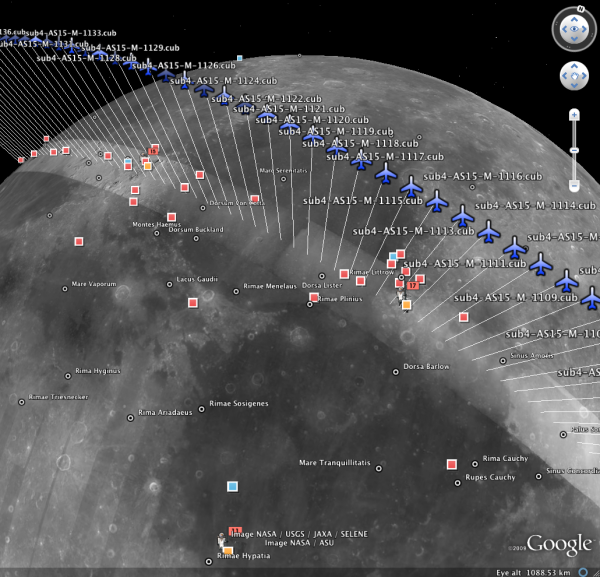
\includegraphics[width=6in]{images/orbitviz_ge_result_600px.png}
  \end{center}
  \caption{ Example of a \ac{KML} visualization produced with {\tt
      orbitviz} depicting camera locations for the Apollo 15 Metric
    Camera during orbit 33 of the Apollo command module.}
  \label{fig:orbitviz_example}
\end{figure}

Usage:
\begin{verbatim}
  orbitviz [options] <input images and cameras> 
\end{verbatim}

\begin{longtable}{|l|p{10cm}|}
\caption{Command-line options for orbitviz}
\label{tbl:orbitviz}
\endfirsthead
\endhead
\endfoot
\endlastfoot
\hline
Options & Description \\ \hline \hline
\texttt{-\/-help|-h} & Display the help message\\ \hline

\texttt{-\/-output|-o \textit{filename(=orbit.kml)}} & The output kml file that will be written \\ \hline

\texttt{-\/-model-scale | -s \textit{float(=1)}} & Scale the size of the coordinate axes by this amount. Ex: To scale axis sizes up to Earth size, use 3.66 \\ \hline

\texttt{-\/-use-path-to-dae-model|-u \textit{fullpath}} & Use this dae model to represent camera location. \emph{Google Sketch up can create these.} \\ \hline

\texttt{-r | -\/-reference-spheroid \textit{string=WGS\_1984}} & Use this reference spheroid (datum). Options: WGS\_1984, D\_MOON (1,737,400 meters), D\_MARS (3,396,190 meters), MOLA (3,396,000 meters), NAD83, WGS72, and NAD27. Also accepted: Earth (=WGS\_1984), Mars (=D\_MARS), Moon (=D\_MOON). \\ \hline

\texttt{-t | -\/-session-type  \textit{string}} & Select the stereo session type to use for processing. Options: pinhole isis spot5 dg aster.\\ \hline

\texttt{-\/-load-camera-solve} & Use a specialized display for showing the results of the \texttt{camera\_solve} tool.
When using this option, only pass in the path to the \texttt{camera\_solve} output folder as a positional argument.
Green lines drawn between the camera positions indicate a successful interest point match between those two images.\\ \hline

\texttt{-\/-hide-labels} & Hide image names unless the camera is highlighted.\\ \hline

\texttt{-\/-bundle-adjust-prefix \textit{string}} & Use the camera adjustment obtained by previously running bundle\_adjust with this output prefix.\\ \hline

\texttt{-\/-write-csv} & Write a csv file with the orbital data.\\ \hline

\end{longtable}

\clearpage

\section{cam2map4stereo.py}
\label{cam2map4stereo}

This program takes similar arguments as the ISIS3 \texttt{cam2map} program,
but takes two input images.  With no arguments, the program determines
the minimum overlap of the two images, and the worst common resolution,
and then map-projects the two images to this identical area and resolution.

The detailed reasons for doing this, and a manual step-by-step walkthrough of
what \texttt{cam2map4stereo.py} does is provided in the discussion on aligning images on page \pageref{sec:AligningImages}.

The \texttt{cam2map4stereo.py} is also useful for selecting a subsection and/or reduced resolution portion of the full image.  You can inspect a raw camera geometry image in qview after you have run \texttt{spiceinit} on it, select the latitude and longitude ranges, and then use \texttt{cam2map4stereo.py}'s \texttt{-\/-lat}, \texttt{-\/-lon}, and optionally \texttt{-\/-resolution} options to pick out just the part you want.

Use the \texttt{-\/-dry-run} option the first few times to get an idea of what \texttt{cam2map4stereo.py} does for you.

\begin{longtable}{|l|p{10cm}|}
\caption{Command-line options for cam2map4stereo.py}
\label{tbl:bundlevis}
\endfirsthead
\endhead
\endfoot
\endlastfoot
\hline
Options & Description \\ \hline \hline
\texttt{-\/-help|-h} & Display the help message. \\ \hline
\texttt{-\/-manual} & Read the manual. \\ \hline
\texttt{-\/-map=\textit{MAP}|-m \textit{MAP}} & The mapfile to use for \texttt{cam2map}. \\ \hline
\texttt{-\/-pixres=\textit{PIXRES}|-p \textit{PIXRES}} & The pixel resolution mode to use for \texttt{cam2map}. \\ \hline
\texttt{-\/-resolution=\textit{RESOLUTION}|-r \textit{RESOLUTION}} & Resolution of the final map for \texttt{cam2map}. \\ \hline
\texttt{-\/-interp=\textit{INTERP}|-i \textit{INTERP}} & Pixel interpolation scheme for \texttt{cam2map}. \\ \hline
\texttt{-\/-lat=\textit{LAT}|-a \textit{LAT}} & Latitude range for \texttt{cam2map}, where \texttt{LAT} is of the form \textit{min:max}.  So to specify a latitude range between -5 and 10 degrees, it would look like \texttt{-\/-lat=-5:10}. \\ \hline
\texttt{-\/-lon=\textit{LON}|-o \textit{LON}} & Longitude range for \texttt{cam2map}, where \texttt{LON} is of the form \textit{min:max}.  So to specify a longitude range between 45 and 47 degrees, it would look like \texttt{-\/-lon=40:47}. \\ \hline
\texttt{-\/-dry-run|-n} & Make calculations, and print the \texttt{cam2map} command that would be executed, but don't actually run it.\\ \hline
\texttt{-\/-prefix} & Make all output files use this prefix. Default: no prefix.\\ \hline
\texttt{-\/-suffix|-s} & Suffix that gets inserted in the output file names, defaults to `map'.\\ \hline
\end{longtable}

\clearpage



\section{pansharp}
\label{pansharp}

This tool reads in a high resolution grayscale file and a low resolution RGB file and produces
a high resolution RGB file.  The output image will be at the resolution of the grayscale image
and will cover the region where the two images overlap.  Both images must have georeferencing
information.  This can either be projection information in the image metadata or it can be a
separate Worldview format XML camera file containing four ground control points
(if using the tool with Digital Globe images).


\medskip

Usage:\\
\hspace*{2em}\texttt{pansharp [options] <grayscale image file> <color image file> <output image file>}

\medskip

\begin{longtable}{|l|p{10cm}|}
\caption{Command-line options for pansharp}
\label{tbl:pansharp}
\endfirsthead
\endhead
\endfoot
\endlastfoot
\hline
Options & Description \\ \hline \hline
\texttt{-\/-help} & Display the help message.\\ \hline
\texttt{-\/-min-value} & Manually specify the bottom of the input data range.\\ \hline
\texttt{-\/-max-value} & Manually specify the top of the input data range.\\ \hline
\texttt{-\/-gray-xml} & Look for georeference data here if not present in the grayscale image.\\ \hline
\texttt{-\/-color-xml} & Look for georeference data here if not present in the RGB image.\\ \hline
\texttt{-\/-nodata-value} & The nodata value to use for the output RGB file.\\ \hline
\end{longtable}

\section{datum\_convert}
\label{datumconvert}

This tool is used to convert a DEM from one datum to another.  For
example, a UTM zone 10 DEM with an NAD27 datum can be converted to a UTM
zone 10 DEM with a WGS84 datum.  This tool does not convert between
projections, another program such as \texttt{gdalwarp} (included with ASP) or
ASP's \texttt{dem\_mosaic} should be used for that. \texttt{datum\_convert} performs both
horizontal and vertical conversion.

Intuitively, the input and output DEMs should correspond to the same
point cloud in 3D space up to the interpolation errors required to
perform the conversion.

\medskip
Usage:\\
\hspace*{2em}\texttt{datum\_convert [options] <input dem> <output dem>}
\medskip

\begin{longtable}{|l|p{10cm}|}
\caption{Command-line options for datum\_convert}
\label{tbl:datumconvert}
\endfirsthead
\endhead
\endfoot
\endlastfoot
\hline
Options & Description \\ \hline \hline
\texttt{-\/-help} & Display the help message.\\ \hline
\texttt{-\/-output-datum \textit{string}} & The datum to convert to. Supported options: WGS\_1984, NAD83, WGS72, and NAD27. \\ \hline
\texttt{-\/-t\_srs \textit{string}} & Specify the output datum via the PROJ.4 string. \\ \hline
\texttt{-\/-nodata-value} & The value of no-data pixels, unless specified in the DEM.\\ \hline
\end{longtable}


\section{point2las}
\label{point2las}

This tool can be used to convert point clouds generated by ASP to the
public LAS format for interchange of 3-dimensional point cloud data.

If the input cloud has a datum, or the \texttt{-\/-datum} option is specified,
then the output LAS file will be created in respect to this datum. Otherwise
raw $x,y,z$ values will be saved.

\begin{longtable}{|l|p{10cm}|}
\caption{Command-line options for point2las}
\label{tbl:point2las}
\endfirsthead
\endhead
\endfoot
\endlastfoot
\hline
Options & Description \\ \hline \hline
\texttt{-\/-help|-h} & Display the help message.\\ \hline
\texttt{-\/-datum} & Create a geo-referenced LAS file in respect to this datum. Options: WGS\_1984, D\_MOON (1,737,400 meters), D\_MARS (3,396,190 meters), MOLA (3,396,000 meters), NAD83, WGS72, and NAD27. Also accepted: Earth (=WGS\_1984), Mars (=D\_MARS), Moon (=D\_MOON). \\ \hline
\texttt{-\/-reference-spheroid \textit{string}} & This is identical to the datum option. \\ \hline
\texttt{-\/-t\_srs \textit{string}} & Specify the output projection (PROJ.4 string). \\ \hline
\texttt{-\/-compressed} &
Compress using laszip. \\ \hline
\texttt{-\/-output-prefix|-o \textit{filename}} & Specify the output file prefix. \\ \hline
\texttt{-\/-threads \textit{integer(=0)}} & Set the number threads to use. 0 means use the default defined in the program or in the .vwrc file.\\ \hline
\texttt{-\/-tif-compress None|LZW|Deflate|Packbits} & TIFF compression method.\\ \hline
\end{longtable}

\section{pc\_align}
\label{pcalign}

This tool can be used to align two point clouds using Point-to-Plane,
Point-to-Point, or Similarity-Point-to-Point Iterative Closest Point
(ICP). (The latter method handles a scale as part of the
alignment transform, not just a rigid transformation.) As an alternative
to ICP, it can use least squares (with outlier handling) to find the
transform, if the reference cloud is a DEM. It uses the
\texttt{libpointmatcher} library~\cite{Pomerleau12comp}
(\url{https://github.com/ethz-asl/libpointmatcher}).

\medskip
Usage:
\begin{verbatim}
  pc_align --max-displacement <float> [other options] <reference cloud> <source cloud> \
    -o <output prefix>}
\end{verbatim}

An example of using this tool is in section \ref{pc-align-example}.

Several important things need to be kept in mind if \texttt{pc\_align} is to be
used successfully and give accurate results, as described below.

\subsection{The input point clouds}

Due to the nature of ICP, the first input point cloud, that is, the
reference (fixed) cloud, should be denser than the second, source (movable)
point cloud, to get the most accurate results. This is not a serious
restriction, as one can perform the alignment this way and then simply
invert the obtained transform if desired (\texttt{pc\_align} outputs
both the direct and inverse transform, and can output the reference
point cloud transformed to match the source and vice-versa).

In many typical applications, the source and reference point clouds are
already roughly aligned, but the source point cloud may cover a larger
area than the reference. The user should provide to \texttt{pc\_align}
the expected maximum distance (displacement) source points may move by
as result of alignment, using the option
\texttt{-\/-max-displacement}. This number will help remove source
points too far from the reference point cloud which may not match
successfully and may degrade the accuracy. If in doubt, this value can
be set to something large but still reasonable, as the tool is able to
throw away a certain number of unmatched outliers. At the end of
alignment, \texttt{pc\_align} will display the {\it observed} maximum
displacement, a multiple of which can be used to seed the tool in a
subsequent run.

The user can choose how many points to pick from the reference and
source point clouds to perform the alignment. The amount of memory and
processing time used by \texttt{pc\_align} is directly proportional to
these numbers, ideally the more points the better. Pre-cropping to
judiciously chosen regions may improve the accuracy and/or run-time.

\subsection{Alignment method}
\label{align-method}

Normally Point-to-Plane ICP is more accurate than Point-to-Point, but
the latter can be good enough if the input point clouds have small
alignment errors and it is faster and uses less memory as well.  The
tool also accepts an option named \texttt{-\/-highest-accuracy} which
will compute the normals for Point-to-Plane ICP at all points rather
than about a tenth of them. This option is not necessary most of the
time, but may result in better alignment at the expense of using more
memory and processing time.

The default alignment transform is rigid, that is, a combination of
rotation and translation. With Point-to-Point ICP, it is also possible
to solve for a scale change (to obtain a so-called \texttt{similarity
transform}). It is suggested this approach be used only when a scale
change is expected. It can be turned on by setting
\texttt{-\/-alignment-method similarity-point-to-point}. 

As an alternative to ICP, least squares (with outlier handling using a
robust cost function) can be used to find the transform, if the
reference cloud is a DEM. For this, one should specify the alignment
method as \texttt{least-squares} or \texttt{similarity-least-squares}
(the latter also solves for scale). This method is somewhat
experimental. It is suggested that the input clouds be very close or
otherwise the \texttt{-\/-initial-transform} option be used, for the
method to converge. Also, fewer iterations than the default may be
needed.

\subsection{File formats}

The input point clouds can be in one of several formats: ASP's point
cloud format (the output of \texttt{stereo}), DEMs as GeoTIFF or ISIS
cub files, LAS files, or plain-text CSV files (with .csv or .txt
extension).

By default, CSV files are expected to have on each line the latitude and
longitude (in degrees), and the height above the datum (in meters),
separated by commas or spaces. Alternatively, the user can specify the
format of the CSV file via the \texttt{-\/-csv-format} option. Entries
in the CSV file can then be (in any order) (a) longitude, latitude (in
degrees), height above datum (in meters), (b) longitude, latitude,
distance from planet center (in meters or km), (c) easting, northing and
height above datum (in meters), in this case a PROJ.4 string must be set
via \texttt{-\/-csv-proj4}, (d) Cartesian coordinates $(x, y, z)$
measured from planet center (in meters). The precise syntax is described
in the table below. The tool can also auto-detect the LOLA RDR
PointPerRow format.

Any line in a CSV file starting with the pound character (\#) is ignored.

If none of the input files have a geoheader with datum information, and
the input files are not in Cartesian coordinates, the datum needs to be
specified via the \texttt{-\/-datum} option, or by setting
\texttt{-\/-semi-major-axis} and \texttt{-\/-semi-minor-axis}.

\subsection{The alignment transform}

The transform obtained by \texttt{pc\_align} is output to a text file as
a $4\times 4$ matrix with the upper-left $3\times 3$ submatrix being the
rotation (and potentially also a scale, per section \ref{align-method}) and
the top three elements of the right-most column being the
translation. This transform, if applied to the source point cloud, will
bring it in alignment with the reference point cloud. The transform
assumes the 3D Cartesian coordinate system with the origin at the planet
center. This matrix can be supplied back to the tool as an initial guess
(section \ref{prevtrans}). The inverse transform is saved to a file as
well.

The \texttt{pc\_align} program outputs the translation component of this
transform, defined as the vector from the centroid of the original
source points to the centroid of the transformed source points. This
translation component is displayed in three ways (a) Cartesian
coordinates with the origin at the planet center, (b) Local
North-East-Down coordinates at the centroid of the original source
points, and (c) Latitude-Longitude-Height differences between the two
centroids. If the effect of the transform is small (e.g., the points
moved by at most several hundred meters) then the representation in the
form (b) above is most amenable to interpretation as it is in respect
to cardinal directions and height above ground if standing at a point on
the planet surface.

The full transform itself, with its origin at the center of the planet,
can result in large movements on the planet surface even for small angles
of rotation. Because of this it may be difficult to interpret both its rotation
and translation components.

\subsection{Applying a previous transform}
\label{prevtrans}

The transform output by \texttt{pc\_align} can be supplied back to the
tool as an initial guess via the \texttt{-\/-initial-transform} option,
with the same or different clouds. If it is desired to simply apply this
transform to the clouds without further work, one can specify
\texttt{-\/-num-iterations 0}.  This may be useful, for example, in
first finding the alignment transform over a smaller, more reliable
region (e.g., over rock, excluding moving ice), then extending it over the entire
available dataset.

\subsection{Error metrics and outliers}

The tool outputs to CSV files the lists of errors together with their
locations in the source point cloud, before and after the alignment of
source points, where an error is defined as the distance from a source
point used in alignment to the closest reference point. The format of
output CSV files is the same as of input CSV files, or as given by
\texttt{-\/-csv-format}, although any columns of extraneous data in the
input files are not saved on output.

The program prints to screen and saves to a log file the 16th, 50th, and
84th error percentiles as well as the means of the smallest 25\%, 50\%,
75\%, and 100\% of the errors.

When the reference point cloud is a DEM, a more accurate computation of
the errors from source points to the reference cloud is used. A source
point is projected onto the datum of the reference DEM, its longitude
and latitude are found, then the DEM height at that position is
interpolated.  That way we determine a ``closest'' point on the
reference DEM that interprets the DEM not just as a collection of points
but rather as a polyhedral surface going through those points. These
errors are what is printed in the statistics. To instead compute
errors as done for other type of point clouds, use the option
\texttt{-\/-no-dem-distances}.

By default, when \texttt{pc\_align} discards outliers during the
computation of the alignment transform, it keeps the 75\% of the points
with the smallest errors. As such, a way of judging the effectiveness of
the tool is to look at the mean of the smallest 75\% of the errors
before and after alignment.

\subsection{Output point clouds and convergence history}

The transformed input point clouds (the source transformed to match the
reference, and the reference transformed to match the source) can also
be saved to disk if desired. If an input point cloud is in CSV or ASP
point cloud format, the output transformed cloud will be in the same
format. If the input is a DEM, the output will be an ASP point cloud,
since a gridded point cloud may not stay so after a 3D transform. The
\texttt{point2dem} program can be used to re-grid the obtained point
cloud back to a DEM.

The convergence history for \texttt{pc\_align} (the translation and
rotation change at each iteration) is saved to disk and can be used to
fine-tune the stopping criteria.

\subsection{Manual alignment}

If automatic alignment fails, for example, if the clouds are too
different, or they differ by a scale factor, manual alignment can be
used instead, either on its own, or as an initial guess for the
automatic alignment transform. For that, the input point clouds should
be first converted to DEMs using \texttt{point2dem}, unless in that
format already. Then, \texttt{stereo\_gui} can be invoked to create
point correspondences (interest point matches) from the reference to the
source DEM. Once these correspondences are saved to a match file,
\texttt{pc\_align} can be called with the reference and source DEMs and
the \texttt{-\/-match-file} option.  This will compute and save to disk
a rotation + translation + scale transform.  A subsequent invocation of
\texttt{pc\_align}, either with the original clouds or the DEM created
from them, can use this transform as an initial guess (section
\ref{prevtrans}).

\subsection{Troubleshooting}

Remember that filtering is applied only to the source point cloud.
If you have an input cloud with a lot of noise, make sure it is
being used as the source cloud.

If you are not getting good results with \texttt{pc\_align}, something
that you can try is to convert an input point cloud into a smoothed DEM.
Use \texttt{point2dem} to do this and set \texttt{-\/-search-radius-factor}
if needed to fill in holes in the DEM.  For some input data this can
significantly improve alignment accuracy.

\medskip

\begin{longtable}{|p{8cm}|p{9cm}|}
\caption{Command-line options for pc\_align}
\label{tbl:pcalign}
\endfirsthead
\endhead
\endfoot
\endlastfoot
\hline
Options & Description \\ \hline \hline
\texttt{-\/-help|-h} & Display the help message.\\ \hline
\texttt{-\/-threads \textit{integer(=0)}} & Set the number threads to
use. 0 means use the default as set by OpenMP. Only some parts of the algorithm are multi-threaded.\\ \hline
\texttt{-\/-initial-transform \textit{string}} &
The file containing the transform to be used as an
initial guess. It can come from a previous run of the tool. \\ \hline
\texttt{-\/-num-iterations \textit{default: 1000}} &  Maximum number of iterations. \\ \hline
\texttt{-\/-diff-rotation-error \textit{default: $10^{-8}$}} & Change in rotation amount below which the algorithm will stop (if translation error is also below bound), in degrees. \\ \hline
\texttt{-\/-diff-translation-error \textit{default: $10^{-3}$}} & Change in translation amount below which the algorithm will stop (if rotation error is also below bound), in meters. \\ \hline
\texttt{-\/-max-displacement \textit{float}} & Maximum expected
displacement of source points as result of alignment, in meters (after
the initial guess transform is applied to the source points). Used
for removing gross outliers in the source (movable) point cloud.\\ \hline
\texttt{-\/-outlier-ratio \textit{default: 0.75}} &  Fraction of source (movable) points considered inliers (after gross outliers further than max-displacement from reference points are removed). \\ \hline
\texttt{-\/-max-num-reference-points \textit{default: $10^8$}} &
Maximum number of (randomly picked) reference points to use. \\ \hline
\texttt{-\/-max-num-source-points \textit{default: $10^5$}} & Maximum number of (randomly picked) source points to use (after discarding gross outliers). \\ \hline
\texttt{-\/-alignment-method \textit{default: point-to-plane}} & The type of iterative closest point method to use. [point-to-plane, point-to-point, similarity-point-to-point, least-squares, similarity-least-squares]\\ \hline
\texttt{-\/-highest-accuracy} & Compute with highest accuracy for point-to-plane (can be much slower). \\ \hline

\texttt{-\/-datum \textit{string}} & Use this datum for CSV files. Options: WGS\_1984, D\_MOON (1,737,400 meters), D\_MARS (3,396,190 meters), MOLA (3,396,000 meters), NAD83, WGS72, and NAD27. Also accepted: Earth (=WGS\_1984), Mars (=D\_MARS), and Moon (=D\_MOON). \\ \hline

\texttt{-\/-semi-major-axis \textit{float}} & Explicitly set the datum semi-major axis in meters.\\ \hline
\texttt{-\/-semi-minor-axis \textit{float}} & Explicitly set the datum semi-minor axis in meters.\\ \hline

\texttt{-\/-csv-format \textit{string}} & Specify the format of input
CSV files as a list of entries column\_index:column\_type (indices start
from 1). Examples: '1:x 2:y 3:z' (a Cartesian coordinate system with
origin at planet center is assumed, with the units being in meters),
'5:lon 6:lat 7:radius\_m' (longitude and latitude are in degrees, the
radius is measured in meters from planet center), '3:lat 2:lon
1:height\_above\_datum', '1:easting 2:northing 3:height\_above\_datum'
(need to set \texttt{-\/-csv-proj4}; the height above datum is in
meters). Can also use radius\_km for column\_type, when it is again
measured from planet center. \\ \hline

\texttt{-\/-csv-proj4 \textit{string}} & The PROJ.4 string to use to
interpret the entries in input CSV files, if those files contain Easting
and Northing fields.  \\ \hline

\texttt{-\/-output-prefix|-o \textit{filename}} & Specify the output file prefix. \\ \hline
\texttt{-\/-compute-translation-only} & Compute the transform from source to reference point cloud as a translation only (no rotation). \\ \hline
\texttt{-\/-save-transformed-source-points} & Apply the obtained transform to the source points so they match the reference points and save them. \\ \hline
\texttt{ -\/-save-inv-transformed-reference-points} & Apply the inverse of the obtained transform to the reference points so they match the source points and save them.
\\ \hline

\texttt{-\/-initial-ned-translation} \textit{string} &  Initialize the alignment transform based on a translation with this vector in the local North-East-Down coordinate system. Specify it in quotes, separated by spaces or commas. \\ \hline

\texttt{-\/-no-dem-distances} & For reference point clouds that are DEMs, don't take advantage of the fact that it is possible to interpolate into this DEM when finding the closest distance to it from a point in the source cloud (the text above has more detailed information). \\ \hline

\texttt{-\/-match-file} & Compute a translation + rotation + scale transform from the source to the reference point cloud using manually selected point correspondences (obtained for example using stereo\_gui). \\ \hline

\texttt{-\/-config-file \textit{file.yaml}} & This is an advanced
option. Read the alignment parameters from a configuration file, in the
format expected by libpointmatcher, over-riding the command-line options.\\ \hline

\end{longtable}

\section{pc\_merge}
\label{pcmerge}

This is a simple tool for combining multiple ASP-generated point cloud files into
a single concatenated file.  The output file will be float32 unless the input images
are float64 or the user has specified the float64 option.

\texttt{pc\_merge} can merge clouds with
1, 3, 4, and 6 bands. In particular, it can merge \textit{output-prefix}-L.tif images
created by \texttt{stereo}. This is useful if it is desired to create an
ortho-image from a merged cloud with \texttt{point2dem}. In that case,
one can invoke \texttt{pc\_merge} on individual ``L'' files to create a
merged texture file to pass to \texttt{point2dem} together with the
merged point cloud tile.


\medskip

Usage:\\
\hspace*{2em}\texttt{pc\_merge [options] [required output file option] <multiple point cloud files>}

\medskip

\begin{longtable}{|l|p{10cm}|}
\caption{Command-line options for pc\_merge}
\label{tbl:pcmerge}
\endfirsthead
\endhead
\endfoot
\endlastfoot
\hline
Options & Description \\ \hline \hline
\texttt{-\/-help} & Display the help message.\\ \hline
\texttt{-\/-write-double|-d} & Force output file to be float64 instead of float32.\\ \hline
\texttt{-\/-output-file|-o} & Specify the output file (required).\\ \hline
\end{longtable}

\section{wv\_correct}
\label{wvcorrect}

An image taken by one of Digital Globe's World View satellite cameras is
formed of several blocks as tall as the image, mosaicked from left to
right, with each block coming from an individual CCD sensor
\cite{digital-globe:camera}. Either due to imperfections in the camera
or in the subsequent processing the image blocks are offset in
respect to each other in both row and column directions by a subpixel
amount. These so-called {\it CCD boundary artifacts} are not visible in
the images but manifest themselves as discontinuities in the the DEMs
obtained with ASP.

The tool named \texttt{wv\_correct} is able to significantly attenuate
these artifacts (see Figure~\ref{fig:ccd-artifact-example} in the
Digital Globe tutorial for an example). This tool should be used on raw
Digital Globe images before calling \texttt{dg\_mosaic} and
\texttt{mapproject}.

It is important to note that both the positions of the CCD offsets and
the offset amounts were determined empirically without knowledge of
Digital Globe's mosaicking process; this is why we are not able to
remove these artifacts completely.

Presently, \texttt{wv\_correct} works for WV01 images for TDI of 8, 16, 32,
48, 56 and 64, and for WV02 images for TDI of 8, 16, 48, and 64 (both the
forward and reverse scan directions for both cameras). In addition, the
WV02 TDI 32 forward scan direction is supported. These are by far the
most often encountered TDI. We plan to extend the tool to support other
TDI when we get more such data to be able to compute the
corrections. For WV03 images, CCD artifacts appear to not be
significant, hence no corrections are planned for the near future.

\medskip

Usage:\\
\hspace*{2em}\texttt{wv\_correct [options] <input image> <input camera model> <output image>}

\medskip

\begin{longtable}{|p{8cm}|p{9cm}|}
\caption{Command-line options for wv\_correct}
\label{tbl:wvcorrect}
\endfirsthead
\endhead
\endfoot
\endlastfoot
\hline
Options & Description \\ \hline \hline
\texttt{-\/-ot \textit{string(=Float32)}} & Output data type. Supported types: Byte, UInt16, Int16, UInt32, Int32, Float32. If the output type is a kind of integer, values are rounded and then clamped to the limits of that type. \\ \hline
\texttt{-\/-help|-h} & Display the help message.\\ \hline
\texttt{-\/-threads \textit{integer(=0)}} & Set the number threads to
use. 0 means use the default defined in the program or in the .vwrc file. \\ \hline
\end{longtable}

\section{lronac2mosaic.py}
\label{lronac2mosaic}

This tool takes in two LRONAC files (M*LE.IMG and M*RE.IMG) and
produces a single noproj mosaic composed of the two inputs.  It
performs the following operations in this process:
\texttt{lronac2isis}, \texttt{lronaccal}, \texttt{lronacecho},
\texttt{spiceinit}, \texttt{noproj}, and \texttt{handmos}. The offsets
used in \texttt{handmos} are calculated using an ASP internal tool
called \texttt{lronacjitreg} and is similar in functionality to the
ISIS command \texttt{hijitreg}. Offsets need to be calculated via
feature measurements in image to correct for imperfections in camera
pointing. The angle between LE and RE optics changes slightly with
spacecraft temperature.

Optionally, \texttt{lronac2mosiac.py} can be given many IMG files all
at once. The tool will then look at image names to determine which
should be paired and mosaicked. The tool will also spawn multiple
processes of ISIS commands were possible to finish the task
faster. The max number of simultaneous processes is limited by the
\texttt{-\/-threads} option.

\medskip

Usage:\\
\hspace*{2em}\texttt{lronac2mosaic.py [options] <IMG file 1> <IMG file 2>}

\medskip

\begin{longtable}{|l|p{10cm}|}
\caption{Command-line options for lronac2mosaic.py}
\label{tbl:lronac2mosaic}
\endfirsthead
\endhead
\endfoot
\endlastfoot
\hline
Options & Description \\ \hline \hline
\texttt{-\/-manual} & Display the help message.\\ \hline
\texttt{-\/-output-dir|-o} & Set the output folder (default is input folder).\\ \hline
\texttt{-\/-stop-at-no-proj} & Stops processing after the noproj steps are complete. \\ \hline
\texttt{-\/-resume-at-no-proj} & Restarts processing using the results from 'stop-at-no-proj. \\ \hline
\texttt{-\/-threads|-t} & Specify the number of threads to use.\\ \hline
\texttt{-\/-keep|-k} & Keep all intermediate files.\\ \hline
\end{longtable}


\section{image\_calc}
\label{imagecalc}

This tool can be used to perform simple, per-pixel arithmetic on one or more
input images. An arithmetic operation specified on the command line is parsed
and applied to each pixel, then the result is written to disk. The tool
supports multiple input images but each must be the same size and data type.
Input images are restricted to one channel.

The following symbols are allowed in the arithmetic string: +, -, *, /,
(), min(), max(), pow(), abs(), and var\_N where N is the index of one
of the input images. An example arithmetic string is: "-abs(var\_2) +
min(58, var\_1, var\_3) / 2".  The tool respects the normal PEMDAS order
of operations \textit{except} that it parses equal priority operations
from right to left, \textit{not} the expected left to right.
Parentheses can be used to enforce any preferred order of evaluation.


\medskip

Usage:
\begin{verbatim}
  image_calc [options] -c <arithmetic formula> <inputs> -o <output>
\end{verbatim}

Example:
\begin{verbatim}
  image_calc -c "pow(var_0/3.0, 1.1)" input_image.tif -o output_image.tif -d float32
\end{verbatim}

\medskip

\begin{longtable}{|l|p{10cm}|}
\caption{Command-line options for image\_calc}
\label{tbl:imagecalc}
\endfirsthead
\endhead
\endfoot
\endlastfoot
\hline
Options & Description \\ \hline \hline
\texttt{-\/-help} & Display the help message.\\ \hline
\texttt{-\/-calc|-c} & The arithmetic string in quotes (required).\\ \hline
\texttt{-\/-output-data-type|-d} & The data type of the output file (default is float64).\\ \hline
\texttt{-\/-input-nodata-value} & Set an override nodata value for the input images.\\ \hline
\texttt{-\/-output-nodata-value} & Manually specify a nodata value for the output image (default is data type min).\\ \hline
\texttt{-\/-output-file|-o} & Specify the output file instead of using a default.\\ \hline
\texttt{-\/-mo \textit{string}} & Write metadata to the output file. Provide as a string in quotes if more than one item, separated by a space, such as 'VAR1=VALUE1 VAR2=VALUE2'. Neither the variable names nor the values should contain spaces. \\ \hline
\end{longtable}

\section{hsv\_merge}
\label{hsvmerge}

Replaces the intensity information in an RGB image with the provided grayscale image
by temporarily converting to HSV.  Both input image must be the same size.

Mimics \texttt{hsv\_merge.py} by Frank Warmerdam and Trent Hare. Use it to combine results from gdaldem.

\medskip

Usage:
\begin{verbatim}
  hsv_merge [options] <rgb_image> <gray_image>
\end{verbatim}

\medskip

\begin{longtable}{|l|p{10cm}|}
\caption{Command-line options for hsv\_merge}
\label{tbl:hsvmerge}
\endfirsthead
\endhead
\endfoot
\endlastfoot
\hline
Options & Description \\ \hline \hline
\texttt{-\/-help} & Display the help message.\\ \hline
\texttt{-\/-output-file|-o} & Specify the output file.  Required!\\ \hline
\end{longtable}


\section{colormap}
\label{sec:colormap}

The \verb#colormap# tool reads a DEM and writes a corresponding color-coded height image that can be used for visualization.


\medskip

Usage:\\
\hspace*{2em}\texttt{colormap [options] <input DEM>}

\medskip


\begin{longtable}{|l|p{10cm}|}
\caption{Command-line options for colormap}
\label{tbl:colormap}
\endfirsthead
\endhead
\endfoot
\endlastfoot
\hline
Option & Description \\ \hline \hline
\verb#--help# & Display a help message. \\ \hline
\verb#-s [ --shaded-relief-file ] arg# & Specify a shaded relief image (grayscale) to apply to the colorized image. \\ \hline
\verb#-o [ --output-file ] arg# & Specify the output file. \\ \hline
\verb#--colormap-style arg# & Specify the colormap style. Options: binary-red-blue (default), jet, or the name of a file having the colormap, similar to the file used by gdaldem. \\ \hline
\verb#--nodata-value arg# & Remap the DEM default value to the min altitude value. \\ \hline
\verb#--min arg# & Minimum height of the color map. \\ \hline
\verb#--max arg# & Maximum height of the color map. \\ \hline
\verb#--moon# & Set the min and max height to good values for the Moon. \\ \hline
\verb#--mars# & Set the min and max height to good values for Mars. \\ \hline
\verb#--legend# & Generate an unlabeled legend, saved as "legend.png". \\ \hline

\end{longtable}

\section{{\tt hillshade}}
\label{sec:hillshade}

The \verb#hillshade# tool reads in a DEM and outputs an image of that
DEM as though it were a three-dimensional surface, with every pixel
shaded as though it were illuminated by a light from a specified
location.

\begin{longtable}{|l|p{11cm}|}
\caption{Command-line options for hillshade}
\label{tbl:hillshade}
\endfirsthead
\endhead
\endfoot
\endlastfoot
\hline
Option & Description \\ \hline \hline
\verb#--help# & Display a help message\\ \hline
\verb#--input-file arg# & Explicitly specify the input file\\ \hline
\verb#-o [ --output-file ] arg# & Specify the output file\\ \hline
\verb#-a [ --azimuth ] arg (=300)# & Sets the direction that the light source is coming from (in degrees).  Zero degrees is to the right, with positive degree counter-clockwise.\\ \hline
\verb#-e [ --elevation ] arg (=20)# & Set the elevation of the light source (in degrees)\\ \hline
\verb#-s [ --scale ] arg (=0)# & Set the scale of a pixel (in the same units as the DTM height values\\ \hline
\verb#--nodata-value arg# & Remap the DEM default value to the min altitude value\\ \hline
\verb#--blur arg# & Pre-blur the DEM with the specified sigma\\ \hline
\end{longtable}

\section{image2qtree}
\label{sec:image2qtree}

\verb#image2qtree# turns a georeferenced image (or images) into a quadtree with geographical metadata.  For example, it can output a kml file for viewing in Google Earth.


\begin{longtable}{|l|p{7.5cm}|}
\caption{Command-line options for image2qtree}
\label{tbl:image2qtree}
\endfirsthead
\endhead
\endfoot
\endlastfoot
\hline
Option & Description \\ \hline \hline
General Options \\ \hline
\verb#--help# & Display a help message\\ \hline
\verb#-o [ --output-name ] arg# & Specify the base output directory\\ \hline
\verb#-q [ --quiet ]# & Quiet output\\ \hline
\verb#-v [ --verbose ]# & Verbose output\\ \hline
\verb#--cache arg (=1024)# & Cache size, in megabytes\\ \hline

Input Options\\ \hline
\verb#--force-wgs84# & Use WGS84 as the input images' geographic coordinate systems, even if they're not (old behavior)\\ \hline
\verb#--pixel-scale arg (=1)# & Scale factor to apply to pixels\\ \hline
\verb#--pixel-offset arg (=0)# & Offset to apply to pixels\\ \hline
\verb#--normalize# & Normalize input images so that their full dynamic range falls in between [0,255]\\ \hline

Output Options\\ \hline
\verb#-m [ --output-metadata ] arg (=none)# & Specify the output metadata type. One of [kml, tms, uniview, gmap, celestia, none]\\ \hline
\verb#--file-type arg (=png)# & Output file type\\ \hline
\verb#--channel-type arg (=uint8)# & Output (and input) channel type. One of [uint8, uint16, int16, float]\\ \hline
\verb#--module-name arg (=marsds)# & The module where the output will be placed. Ex: marsds for Uniview, or Sol/Mars for Celestia\\ \hline
\verb#--terrain# & Outputs image files suitable for a Uniview terrain view. Implies output format as PNG, channel type uint16. Uniview only\\ \hline
\verb#--jpeg-quality arg (=0.75)# & JPEG quality factor (0.0 to 1.0)\\ \hline
\verb#--png-compression arg (=3)# & PNG compression level (0 to 9)\\ \hline
\verb#--palette-file arg# & Apply a palette from the given file\\ \hline
\verb#--palette-scale arg# & Apply a scale factor before applying the palette\\ \hline
\verb#--palette-offset arg# & Apply an offset before applying the palette\\ \hline
\verb#--tile-size arg (=256)# & Tile size, in pixels\\ \hline
\verb#--max-lod-pixels arg (=1024)# & Max LoD in pixels, or -1 for none (kml only)\\ \hline
\verb#--draw-order-offset arg (=0)# & Offset for the <drawOrder> tag for this overlay (kml only)\\ \hline
\verb#--composite-multiband # & Composite images using multi-band blending\\ \hline
\verb#--aspect-ratio arg (=1)# & Pixel aspect ratio (for polar overlays; should be a power of two)\\ \hline

Projection Options\\ \hline
\verb#--north arg# & The northernmost latitude in degrees\\ \hline
\verb#--south arg# & The southernmost latitude in degrees\\ \hline
\verb#--east arg# & The easternmost longitude in degrees\\ \hline
\verb#--west arg# & The westernmost longitude in degrees\\ \hline
\verb#--force-wgs84# & Assume the input images' geographic coordinate systems are WGS84, even if they're not (old behavior)\\ \hline
\verb#--sinusoidal# & Assume a sinusoidal projection\\ \hline
\verb#--mercator# & Assume a Mercator projection\\ \hline
\verb#--transverse-mercator# & Assume a transverse Mercator projection\\ \hline
\verb#--orthographic# & Assume an orthographic projection\\ \hline
\verb#--stereographic# & Assume a stereographic projection\\ \hline
\verb#--lambert-azimuthal# & Assume a Lambert azimuthal projection\\ \hline
\verb#--lambert-conformal-conic# & Assume a Lambert Conformal Conic projection\\ \hline
\verb#--utm arg# & Assume UTM projection with the given zone\\ \hline
\verb#--proj-lat arg# & The center of projection latitude (if applicable)\\ \hline
\verb#--proj-lon arg# & The center of projection longitude (if applicable)\\ \hline
\verb#--proj-scale arg# & The projection scale (if applicable)\\ \hline
\verb#--std-parallel1 arg# & Standard parallels for Lambert Conformal Conic projection\\ \hline
\verb#--std-parallel2 arg# & Standard parallels for Lambert Conformal Conic projection\\ \hline
\verb#--nudge-x arg# & Nudge the image, in projected coordinates\\ \hline
\verb#--nudge-y arg# & Nudge the image, in projected coordinates\\ \hline
\end{longtable}

\section{geodiff}
\label{geodiff}

The \texttt{geodiff} program takes as input two DEMs (or a DEM and a CSV file, with the latter in the same format as used for \texttt{pc\_align} and \texttt{point2dem}), and subtracts the second from the first. The grid used is the one from the first DEM, so the second one is interpolated into it (when one file is a CSV, the grid from the second one, the DEM, is used). The tool can also take the absolute difference of the two DEMs.

It is important to note that the tool is very sensitive to the order of
the two DEMs, due to the fact that the grid comes from the first
one. Ideally the grid of the first DEM would be denser than the one of
the second.

\medskip

Usage:
\begin{verbatim}
  > geodiff [options] <dem1> <dem2> [ -o output_file_prefix ]
\end{verbatim}

\begin{longtable}{|l|p{7.5cm}|}
\caption{Command-line options for geodiff}
\label{tbl:geodiff}
\endfirsthead
\endhead
\endfoot
\endlastfoot
\hline
Option & Description \\ \hline \hline
\texttt{-\/-help|-h} & Display the help message. \\ \hline
\texttt{-\/-output-prefix|-o \textit{filename}} & Specify the output prefix. \\ \hline
\texttt{-\/-absolute} & Output the absolute difference as opposed to just the difference. \\ \hline
\texttt{-\/-float} & Output using float (32 bit) instead of using doubles (64 bit). \\ \hline
\texttt{-\/-csv-format \textit{string}} & Specify the format of input
CSV files as a list of entries column\_index:column\_type (indices start
from 1). Examples: '1:x 2:y 3:z' (a Cartesian coordinate system with
origin at planet center is assumed, with the units being in meters),
'5:lon 6:lat 7:radius\_m' (longitude and latitude are in degrees, the
radius is measured in meters from planet center), '3:lat 2:lon
1:height\_above\_datum', '1:easting 2:northing 3:height\_above\_datum'
(need to set \texttt{-\/-csv-proj4}; the height above datum is in
meters). Can also use radius\_km for column\_type, when it is again
measured from planet center. \\ \hline

\texttt{-\/-csv-proj4 \textit{string}} & The PROJ.4 string to use to
interpret the entries in input CSV files, if those files contain Easting
and Northing fields. If not specified, it will be
borrowed from the DEM. \\ \hline

\texttt{-\/-nodata-value \textit{float(=-32768)}} & The no-data value to use, unless present in the DEM geoheaders. \\ \hline
\texttt{-\/-threads \textit{integer(=0)}} & Set the number of threads to use. 0 means use as many threads as there are cores.\\ \hline
\texttt{-\/-no-bigtiff} & Tell GDAL to not create bigtiffs.\\ \hline
\texttt{-\/-tif-compress None|LZW|Deflate|Packbits} & TIFF compression method.\\ \hline
\hline
\end{longtable}


\section{aster2asp}
\label{app:aster}

The \texttt{aster2asp} tool takes as input a directory containing ASTER images and associated 
metadata, and creates TIF and XML files that can then be passed to \texttt{stereo} to create
a point cloud. 

An example for how to use this tool is given in section \ref{sec:aster}.

The tool can only process Level 1A ASTER images. The input should be a
directory containing visible and near-infrared (VNIR) nadir (Band3N) and
backward (Band3B) images, together with plain text files containing
values for the satellite positions, sight vectors, longitudes,
latitudes, lattice points, and radiometric correction tables. These
files are described in \cite{abrams2002aster}.

Usage:
\begin{verbatim}
  aster2asp <input directory> -o <output prefix>
\end{verbatim}

The tool will apply the existing radiometric corrections to the the
images, and save two images with Float32 pixels with names like
\texttt{out-Band3N.tif} and \texttt{out-Band3B.tif}. Based on the
metadata mentioned earlier, it will create approximate RPC camera models
in XML format (section \ref{rpc}) for the left and right cameras,
following \cite{girod2015improvement}, with names of the form
\texttt{out-Band3N.xml} and \texttt{out-Band3B.xml} (we do not perform
yet any jitter corrections as described in that paper).

These can then be passed to \texttt{stereo} as:
\begin{verbatim}
  stereo -t rpc out-Band3N.tif out-Band3B.tif out-Band3N.xml out-Band3B.xml \ 
     out_stereo/run
\end{verbatim}

It is important to note that the tool expects the minimum and maximum
simulation box heights (in meters, above the datum) in which to compute
the RPC approximation. The defaults are 0 and 8000, corresponding to sea
level and the highest location on Earth. Narrowing down these numbers
(if it is known what range of terrain heights is expected) may result in
slightly more accurate models.

\begin{longtable}{|l|p{7.5cm}|}
\caption{Command-line options for aster2asp}
\label{tbl:aster2asp}
\endfirsthead
\endhead
\endfoot
\endlastfoot
\hline
Option & Description \\ \hline \hline
\texttt{-o | -\/-output-prefix  arg} & Specify the output prefix.\\ \hline
\texttt{-\/-min-height arg (=0)} & The minimum height (in meters) above the WGS84 datum of the simulation box in which to compute the RPC approximation.\\ \hline
\texttt{-\/-max-height arg (=8000)} & The maximum height (in meters) above the WGS84 datum of the simulation box in which to compute the RPC approximation.\\ \hline
\texttt{-\/-num-samples arg (=100)} & How many samples to use between the minimum and maximum heights.\\ \hline
\texttt{-\/-penalty-weight arg (=0.1)} & Penalty weight to use to keep the higher-order RPC coefficients small. Higher penalty weight results in smaller such coefficients.\\ \hline
\texttt{-\/-no-bigtiff} & Tell GDAL to not create bigtiffs.\\ \hline
\texttt{-\/-tif-compress arg (=LZW)} & TIFF Compression method. [None, LZW, Deflate, Packbits]\\ \hline
\texttt{-v | -\/-version } & Display the version of software.\\ \hline
\texttt{-h | -\/-help } & Display this help message.\\ \hline
\end{longtable}


\section{add\_spot\_rpc}
\label{app:addspotrpc}

The \texttt{add\_spot\_rpc} tool creates an RPC model to approximate a
SPOT5 sensor model.  The RPC model can be appended to the end of a
SPOT5 metadata file, allowing it to be used with the RPC session type
in other ASP tools.  The most important application is to map project
SPOT5 images, then to perform stereo on the map projected images with
the \texttt{spot5maprpc} session type.

If the output file does not exist, a new file is created containing the
RPC model.  Otherwise the RPC model is appended to an existing file.
When an existing SPOT5 metadata file is the output file, the new RPC
model is properly inserted into the file so that it is ready to use.

An example for how to use this tool is given in section \ref{sec:spot5}.


Usage:
\begin{verbatim}
  add_spot_rpc <input metadata file> -o <output file>
\end{verbatim}

It is important to note that the tool expects the minimum and maximum
simulation box heights (in meters, above the datum) in which to compute
the RPC approximation. The defaults are 0 and 8000, corresponding to sea
level and the highest location on Earth. Narrowing down these numbers
(if it is known what range of terrain heights is expected) may result in
slightly more accurate models.

\begin{longtable}{|l|p{7.5cm}|}
\caption{Command-line options for add\_spot\_rpc}
\label{tbl:addspotrpc}
\endfirsthead
\endhead
\endfoot
\endlastfoot
\hline
Option & Description \\ \hline \hline
\texttt{-o | -\/-output-prefix  arg} & Specify the output prefix.\\ \hline
\texttt{-\/-min-height arg (=0)} & The minimum height (in meters) above the WGS84 datum of the simulation box in which to compute the RPC approximation.\\ \hline
\texttt{-\/-max-height arg (=8000)} & The maximum height (in meters) above the WGS84 datum of the simulation box in which to compute the RPC approximation.\\ \hline
\texttt{-\/-num-samples arg (=100)} & How many samples to use between the minimum and maximum heights.\\ \hline
\texttt{-\/-penalty-weight arg (=0.1)} & Penalty weight to use to keep the higher-order RPC coefficients small. Higher penalty weight results in smaller such coefficients.\\ \hline
\texttt{-v | -\/-version } & Display the version of software.\\ \hline
\texttt{-h | -\/-help } & Display this help message.\\ \hline
\end{longtable}


\section{sfs}
\label{sfs}

The \texttt{sfs} tool can improve a DEM using
shape-from-shading. Examples for how to use it are in chapter
\ref{ch:sfs}. The tool \texttt{parallel\_sfs} (next section) extends
\texttt{sfs} to run using multiple processes and potentially on multiple
machines.

Usage:
\begin{verbatim}
  sfs -i <input DEM> -n <max iterations> -o <output prefix> <images> [other options]
\end{verbatim}

The tool outputs at each iteration the current DEM and a slew of other auxiliary and 
appropriately-named datasets.

\begin{longtable}{|l|p{7.5cm}|}
\caption{Command-line options for sfs}
\label{tbl:sfs}
\endfirsthead
\endhead
\endfoot
\endlastfoot
\hline
Option & Description \\ \hline \hline
\texttt{-i | -\/-input-dem  arg} & The input DEM to refine using SfS.\\ \hline
\texttt{-o | -\/-output-prefix  arg} & Prefix for output filenames.\\ \hline
\texttt{-n | -\/-max-iterations  arg (=100)} & Set the maximum number of iterations.\\ \hline
\texttt{-\/-reflectance-type arg (=1)} & Reflectance type (0 = Lambertian, 1 = Lunar-Lambert, 2 = Hapke, 3 = Experimental extension of Lunar-Lambert, 4 = Charon model (a variation of Lunar-Lambert)).\\ \hline
\texttt{-\/-smoothness-weight arg (=0.04)} & A larger value will result in a smoother solution.\\ \hline
\texttt{-\/-initial-dem-constraint-weight arg (=0)} & A larger value will try harder to keep the SfS-optimized DEM closer to the initial guess DEM.\\ \hline
\texttt{-\/-albedo-constraint-weight arg (=0)} & If floating the albedo, a larger value will try harder to keep the optimized albedo close to the nominal value of 1.\\ \hline
\texttt{-\/-bundle-adjust-prefix arg} & Use the camera adjustments obtained by previously running bundle\_adjust with this output prefix.\\ \hline
\texttt{-\/-float-albedo} & Float the albedo for each pixel. Will give incorrect results if only one image is present.\\ \hline
\texttt{-\/-float-exposure} & Float the exposure for each image. Will give incorrect results if only one image is present.\\ \hline
\texttt{-\/-float-cameras} & Float the camera pose for each image except the first one.\\ \hline
\texttt{-\/-float-all-cameras} & Float the camera pose for each image, including the first one. Experimental.\\ \hline
\texttt{-\/-model-shadows} & Model the fact that some points on the DEM are in the shadow (occluded from the Sun).\\ \hline
\texttt{-\/-shadow-thresholds arg} & Optional shadow thresholds for the input images (a list of real values in quotes, one per image).\\ \hline
\texttt{-\/-save-dem-with-nodata} & Save a copy of the DEM while using a no-data value at a DEM grid point where all images show shadows. To be used if shadow thresholds are set.\\ \hline
\texttt{-\/-use-approx-camera-models} & Use approximate camera models for speed.\\ \hline
\texttt{-\/-use-rpc-approximation} & Use RPC approximations for the camera models instead of approximate tabulated camera models (invoke with --use-approx-camera-models).\\ \hline
\texttt{-\/-rpc-penalty-weight arg (=0.1)} & The RPC penalty weight to use to keep the higher-order RPC coefficients small, if the RPC model approximation is used. Higher penalty weight results in smaller such coefficients.\\ \hline
\texttt{-\/-coarse-levels arg (=0)} & Solve the problem on a grid coarser than the original by a factor of 2 to this power, then refine the solution on finer grids. Experimental.\\ \hline
\texttt{-\/-max-coarse-iterations arg (=50)} & How many iterations to do at levels of resolution coarser than the final result.\\ \hline
\texttt{-\/-crop-input-images} & Crop the images to a region that was computed to be large enough and keep them fully in memory, for speed.\\ \hline
\texttt{-\/-image-exposures-prefix arg} & Use this prefix to optionally read initial exposures (filename is <prefix>-exposures.txt).\\ \hline
\texttt{-\/-model-coeffs-prefix arg} & Use this prefix to optionally read model coefficients from a file (filename is <prefix>-model\_coeffs.txt) .\\ \hline
\texttt{-\/-model-coeffs arg} & Use the model coefficients specified as a list of numbers in quotes. Lunar-Lambertian: O, A, B, C, e.g., '1 0.019 0.000242 -0.00000146'. Hapke: omega, b, c, B0, h, e.g., '0.68 0.17 0.62 0.52 0.52'. Charon: A, f(alpha), e.g., '0.7 0.63'.\\ \hline
\texttt{-\/-crop-win arg (=xoff yoff xsize ysize)} & Crop the input DEM to this region before continuing.\\ \hline
\texttt{-\/-init-dem-height arg (=nan)} & Use this value for initial DEM heights. An input DEM still needs to be provided for georeference information.\\ \hline
\texttt{-\/-nodata-value arg (=nan)} & Use this as the DEM no-data value, over-riding what is in the initial guess DEM.\\ \hline
\texttt{-\/-float-dem-at-boundary} & Allow the DEM values at the boundary of the region to also float (not advised).\\ \hline
\texttt{-\/-fix-dem} & Do not float the DEM at all. Useful when floating the model params.\\ \hline
\texttt{-\/-float-reflectance-model} & Allow the coefficients of the reflectance model to float (not recommended).\\ \hline
\texttt{-\/-query} & Print some info and exit. Invoked from parallel\_sfs.\\ \hline
\texttt{-\/-camera-position-step-size arg (=1)} & Larger step size will result in more aggressiveness in varying the camera position if it is being floated (which may result in a better solution or in divergence).\\ \hline
\texttt{-\/-threads arg (=0)} & Select the number of processors (threads) to use.\\ \hline
\texttt{-\/-no-bigtiff} & Tell GDAL to not create bigtiffs.\\ \hline
\texttt{-\/-tif-compress arg (=LZW)} & TIFF Compression method. [None, LZW, Deflate, Packbits]\\ \hline
\texttt{-v | -\/-version } & Display the version of software.\\ \hline
\texttt{-h | -\/-help } & Display this help message.\\ \hline
\end{longtable}

\section{parallel\_sfs}
\label{psfs}

The program \texttt{parallel\_sfs} is a wrapper around \texttt{sfs}
meant to divide the input DEM into tiles with overlap, run \texttt{sfs} 
on each tile as multiple processes, potentially on multiple machines,
and then merge the results into a single output DEM. It has the same
options as \texttt{sfs}, and a few additional ones, as outlined below.

Usage:
\begin{verbatim}
  parallel_sfs -i <input DEM> -n <max iterations> -o <output prefix> <images> [other options]
\end{verbatim}

\begin{longtable}{|l|p{7.5cm}|}
\caption{Command-line options for parallel\_sfs}
\label{tbl:parallel_sfs}
\endfirsthead
\endhead
\endfoot
\endlastfoot
\hline
Option & Description \\ \hline \hline
\texttt{-\/-tile-size (integer=300)} & Size of approximately square tiles to break up processing into (not counting the padding).\\ \hline
\texttt{-\/-padding (integer=50)} & How much to expand a tile in each direction. This helps with reducing artifacts in the final mosaicked SfS output.\\ \hline
\texttt{-\/-num-processes integer} & Number of processes to use (the default program tries to choose best). \\ \hline
\texttt{-\/-nodes-list string} & A file containing the list of computing nodes, one per line. If not provided, run on the local machine.\\ \hline
\texttt{-\/-threads (integer=1)} & How many threads each process should use. The sfs executable is single-threaded in most of its execution, so a large number will not help here.\\ \hline
\texttt{-\/-suppress-output} & Suppress output of sub-calls.\\ \hline
\end{longtable}


\section{undistort\_image}
\label{undistortimage}

The \texttt{undistort\_image} program takes as input an image and a pinhole model .tsai file
describing the image.  The tool will generate a copy of the input image with the lens distortion
specified in the pinhole model file removed. It will also save the corresponding pinhole
camera model file without the distortion. 

Usage:
\begin{verbatim}
  > undistort_image [options] <input image> <camera model> -o <output image>
\end{verbatim}

\begin{longtable}{|l|p{7.5cm}|}
\caption{Command-line options for undistort\_image}
\label{tbl:undistortimage}
\endfirsthead
\endhead
\endfoot
\endlastfoot
\hline
Option & Description \\ \hline \hline
\texttt{-\/-help|-h} & Display the help message. \\ \hline
\texttt{-\/-output-file|-o \textit{filename}} & Specify the output file. \\ \hline
\texttt{-\/-output-nodata-value \textit{double(=smallest float)}} & 
Set the output nodata value. Only applicable if the output is a single-channel 
image with pixels that are float or double.  \\ \hline

\texttt{-\/-preserve-pixel-type} & 
Save the undistorted image with integer pixels if so is the input. This may 
result in reduced accuracy.
\\ \hline

\texttt{-\/-interpolation-method \textit{string}} & 
Interpolation method. Options: bilinear, bicubic. Default: bilinear. 
\\ \hline

\end{longtable}

\section{camera\_calibrate}
\label{cameracalibrate}

The \texttt{camera\_calibrate} tool can generate camera models suitable for use by \texttt{camera\_solve}
and other ASP tools.  This tool only solves for intrinsic camera parameters; to obtain the camera pose you
should  use the \texttt{camera\_solve} tool.  This tool is a wrapper around the OpenCV (\url{http://opencv.org/})
checkerboard calibration tool which takes care of converting the output into readily usable formats.  When you
run the tool, three camera model files will be created in the output folder:
\texttt{solve\_cam\_params.txt}, \texttt{vw\_cam\_params.tsai}, and \texttt{ocv\_cam\_params.yml}.
The first file can be used as a camera calibration file for the \texttt{camera\_solve} tool.  The second file
is a pinhole camera format that is recognized by ASP but remember that the extrinsic parameters were not solved
for so ASP is limited in what it can do with the camera file.  The last file contains the camera information as
formatted by the OpenCV calibration tool.  If you use the first file as an input to \texttt{camera\_solve}
you must remember to replace the wildcard image path in the file with the one to the images you want to use
solve for (as opposed to the checkerboard images).

In order to use this tool you must provide multiple images of the same checkerboard pattern acquired with
the camera you wish to calibrate.  When calling the tool you must specify the number of internal square corners
contained in your checkerboard pattern (width and height can be swapped) so that OpenCV knows what to look for.
You must also specify an image wildcard path such as \texttt{"checkers/image\_*.jpg"}.  You may need to enclose this
parameter in quotes so that your command line does not expand the wildcard before it is passed to the tool.
If you do not provide the \texttt{--box-size} parameter the output calibration numbers will be unitless.

Usage:
\begin{verbatim}
  > camera_calibrate [options] <output folder> <Board Height> <Board Width> <Image Wildcard> ...
\end{verbatim}

\begin{longtable}{|l|p{7.5cm}|}
\caption{Command-line options for camera\_calibrate}
\label{tbl:cameracalibrate}
\endfirsthead
\endhead
\endfoot
\endlastfoot
\hline
Option & Description \\ \hline \hline
\texttt{-h | -\/-help } & Display this help message.\\ \hline
\texttt{-\/-overwrite}  & Recompute any intermediate steps already completed on disk.\\ \hline
\texttt{-\/-suppress-output} & Reduce the amount of program console output.\\ \hline
\texttt{-\/-box-size-cm  \textit{float}} & The size of the checkerboard squares in centimeters.\\ \hline
\texttt{-\/-duplicate-files} & Make a copy of the vw param file for each input camera.\\ \hline
\end{longtable}

\section{camera\_solve}
\label{camerasolve}

The \texttt{camera\_solve} tool generates pinhole sensor models (frame
cameras), including camera poses, for input images lacking metadata.  See chapter
\ref{ch:sfm} for an overview and examples of using the tool.

The camera calibration passed with the \texttt{-\/-calib-file} option
 should be a .tsai pinhole camera model file in one of the formats
compatible with ASP.  Our supported pinhole camera models are described
in appendix \ref{chapter:pinholemodels}.


You can use a set of estimated camera positions to register
camera models in world coordinates.
This method is not as accurate as using ground control points but it may
be easier to use.  To do this, use the \texttt{-\/-camera-positions} parameter to
\texttt{bundle-adjust} via the \texttt{-\/-bundle-adjust-params} option similar to
the example line below.  If you see the camera models shifting too far from their
starting positions try using the \texttt{-\/-camera-weight} option to restrain
their movement.

\begin{verbatim}
--bundle-adjust-params '--camera-positions nav.csv \
 --csv-format "1:file 12:lat 13:lon 14:height_above_datum" --camera-weight 1.0'
\end{verbatim}

This tool will generate two .tsai camera model files in the output folder per input image.
The first file, appended with .tsai, is in a local coordinate system and does not include
optimizations for intrinsic parameters but it may be useful for debugging purposes.
The second file, appended with .final.tsai, contains the final solver results.  If ground control points or
estimated camera positions were provided then the second file will be in a global coordinate system.


Usage:
\begin{verbatim}
  > camera_solve [options] <output folder> <Input Image 1> <Input Image 2> ...
\end{verbatim}

\begin{longtable}{|l|p{7.5cm}|}
\caption{Command-line options for camera\_solve}
\label{tbl:camerasolve}
\endfirsthead
\endhead
\endfoot
\endlastfoot
\hline
Option & Description \\ \hline \hline
\texttt{-h | -\/-help } & Display this help message.\\ \hline
\texttt{-\/-datum  \textit{string}} & The datum to use when calibrating.  Default is WGS84.\\ \hline
\texttt{-\/-calib-file  \textit{string}} & Path to an ASP compatible pinhole model file containing 
camera model information. The position and pose information will be ignored. If you want 
to use a unique file for each input image, pass a space separated list of files surrounded by quotes.\\ \hline
\texttt{-\/-gcp-file  \textit{string}} & Path to a ground control point file.  This allows
the tool to generate cameras in a global coordinate system.\\ \hline
\texttt{-\/-bundle-adjust-params  \textit{string}} & Additional parameters (in single quotes)
to pass to the \texttt{bundle\_adjust} tool.\\ \hline
\texttt{-\/-theia-flagfile  \textit{string}} & Path to a custom Theia flagfile to use settings from.
File paths specified in this file are ignored.\\ \hline
\texttt{-\/-overwrite}  & Recompute any intermediate steps already completed on disk.\\ \hline
\texttt{-\/-reuse-theia-matches}  & Pass Theia's IP find results into ASP instead of recomputing 
them to reduce total processing time.\\ \hline
\texttt{-\/-suppress-output} & Reduce the amount of program console output.\\ \hline
% \texttt{-i | -\/-solve-intrinsics  \textit{false}} & Try to solve for the camera intrinsic parameters.  If
%not set, the tool will just use the provided camera parameters.  If calib-file is not set then this will be
%set to true.\\
\end{longtable}

This tool is a wrapper that relies on on two other tools to operate.
The first of these is THEIA, as mentioned earlier, for computing the
relative poses of the cameras.  ASP's \texttt{bundle\_adjust} tool is
used to register the cameras in world coordinates using the ground
control points.  If the tool does not provide good results you can
customize the parameters being passed to the underlying tools in order
to improve the results.  For \texttt{bundle\_adjust} options, see the
description in this document.  For more information about THEIA flagfile
options see their website or edit a copy of the default flagfile
generated in the output folder

\section{convert\_pinhole\_model}
\label{convertpinholemodel}

This tool can be used to approximately convert a pinhole model from one
of the types listed in chapter \ref{chapter:pinholemodels} to any other
type. This can be convenient, for example, because the Brown-Conrady and Photometrix models
provide a fast formula to undistort pixels, while the distortion operation is very slow,
requiring a solver with multiple iterations using the undistortion formula at each step,
which can make it time-consuming to run bundle adjustment and epipolar alignment during stereo.
For other models, such as Tsai and Adjustable Tsai, the reverse is true, hence converting
from the former to the latter models can be very convenient for performance reasons. 

Also, this tool can be used to convert a pinhole model to one with RPC
lens distortion (chapter \ref{chapter:pinholemodels}), which is a model
with many more coefficients, and later its coefficients can be optimized
using bundle adjustment to refine the distortion coefficients (section \ref{floatingintrinsics}). 


Usage:
\begin{verbatim}
  > convert_pinhole_model [options] <input image> <input camera> -o <output camera>
\end{verbatim}

\begin{longtable}{|l|p{7.5cm}|}
\caption{Command-line options for camera\_solve}
\label{tbl:camerasolve}
\endfirsthead
\endhead
\endfoot
\endlastfoot
\hline
Option & Description \\ \hline \hline
\texttt{-h | -\/-help } & Display this help message.\\ \hline

\texttt{-o | -\/-output-file \textit{string} } & Specify the output file. It is expected to have the .tsai extension. \\ \hline

\texttt{-\/-output-type \textit{string}} & The output model type. Options: TsaiLensDistortion, 
BrownConradyDistortion, RPC, RPC5, RPC6. Default: TsaiLensDistortion.\\ \hline

\texttt{-\/-sample-spacing \textit{int}} & Pick one out of this many
consecutive pixels to sample. Default: 50. \\ \hline

\end{longtable}

\section{icebridge\_kmz\_to\_csv}
\label{icebridgekmztocsv}

A simple tool for use with data from the NASA IceBridge program.  Google Earth compatible
.kmz files are available at \url{http://asapdata.arc.nasa.gov/dms/missions.html} which display
the aircraft position at the point when each DMS frame image was captured.  This tool exports
those positions into a csv file which can be passed into \texttt{bundle\_adjust} using
the following parameters:
\begin{verbatim}
--camera-positions ../camera_positions.csv --csv-format "1:file 2:lon 3:lat 4:height_above_datum"
\end{verbatim}
This may be useful in conjunction with the \texttt{camera\_solve} tool to allow conversion of camera
positions from local to global coordinates.

Usage:
\begin{verbatim}
  > icebridge_kmz_to_csv <input kmz file> <output csv file>
\end{verbatim}



\section{lvis2kml}
\label{lvis2kml}

A simple tool for use with LVIS (Land, Vegetation, and Ice Sensor) lidar data from the
NASA IceBridge program.  Generates a Google Earth compatible .kml files from either
an LVIS data file (.TXT extension) or an LVIS boundary file (.xml extension).  Using
this tool makes it easy to visualize what region a given LVIS file covers and what
the shape of its data looks like.  If the output path is not passed to the tool it
will generate an output path by appending ".kml" to the input path.  This tool requires
the simplekml Python package to run.  One way to get this is to install the ASP Python
tools, described at the end of section \ref{sparse-disp}.

Usage:
\begin{verbatim}
  > lvis2kml [options] <input path> [output path]
\end{verbatim}


\begin{longtable}{|l|p{7.5cm}|}
\caption{Command-line options for lvis2kml}
\label{tbl:lvis2kml}
\endfirsthead
\endhead
\endfoot
\endlastfoot
\hline
Option & Description \\ \hline \hline
\texttt{-h | -\/-help } & Display this help message.\\ \hline
\texttt{-\/-name  \textit{string}} & Assign a name to the KML file.\\ \hline
\texttt{-\/-color  \textit{string}} & Draw plots in one of (red | green | blue)\\ \hline
\texttt{-\/-skip  \textit{int(=1)}} & When loading a data file, plot only every N-th point.
Has no effect on boundary files.\\ \hline
\end{longtable}

\begin{figure}[!b]
  \begin{center}
  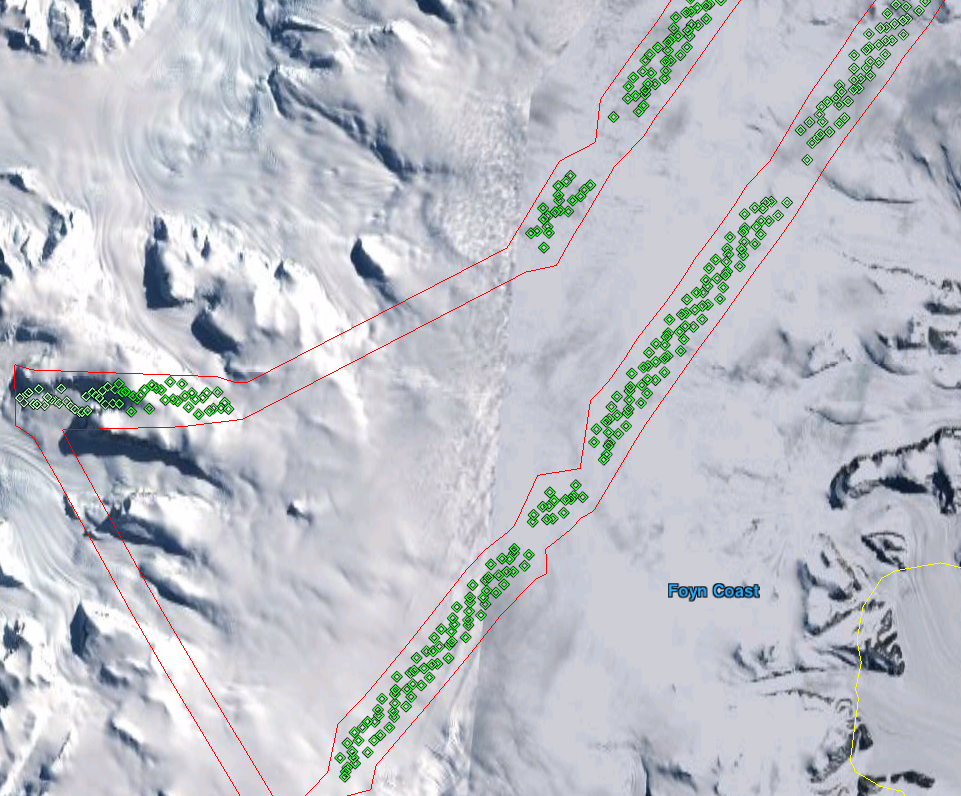
\includegraphics[width=6in]{images/lvis2kml_snap.png}
  \end{center}
  \caption{ Example of \ac{KML} visualizations produced with {\tt
      lvis2kml}.  The output from both the boundary file (red) and the data file
      (green) with a point skip of 500 are shown in this image.  The color saturation of
      data points is scaled with the elevation such that the points in the file with the least
      elevation show up as white and the highest points show up as the specified color.}
  \label{fig:lvis2kml_example}
\end{figure}


\section{GDAL Tools}

ASP distributes in the \texttt{bin} directory the following GDAL tools:
\texttt{gdalinfo}, \texttt{gdal\_translate}, \texttt{gdalbuildvrt}, \texttt{gdalwarp}, 
and \texttt{gdaldem}.
These executables are compiled with
JPEG2000 and BigTIFF support, and can handle NTF images in addition to
most image formats.  They can be used to see image statistics, crop and
scale images, build virtual mosaics, reproject DEMs, etc. Detailed
documentation is available on the GDAL web site, at
\url{http://www.gdal.org/}.
